% -*- TeX:UTF-8 -*-
%%
%% KAIST 학위논문양식 LaTeX용 (ver 0.5) 예시
%%
%% @version 0.4
%% @author  채승병 Chae,Seungbyung (mailto:chess@kaist.ac.kr)
%% @date    2004. 11. 12.
%%
%% @requirement
%% teTeX, fpTeX, teTeX 등의 LaTeX2e 배포판
%% + 은광희 님의 HLaTeX 0.991 이상 버젼 또는 홍석호 님의 HPACK 1.0
%% : 설치에 대한 자세한 정보는 http://www.ktug.or.kr을 참조바랍니다.
%%
%% @note
%% 기존에 널리 쓰여오던 차재춘 님의 학위논문양식 클래스 파일의 형식을
%% 따르지 않고 전면적으로 다시 작성하였습니다. 논문 정보 입력부분에서
%% 과거 양식과 다른 부분이 많으니 아래 예시에 맞춰 바꿔주십시오.
%%
%%
%% @acknowledgement
%% 본 예시 논문은 물리학과 박사과정 김용현 님의 호의로 제공되었습니다.
%%
%% -------------------------------------------------------------------
%% @information
%% 이 예제 파일은 hangul-ucs를 사용합니다. UTF-8 입력 인코딩으로
%% 작성되었습니다. hlatex의 hfont는 이용하지 않습니다. --2006/02/11
%% 본 템플릿은 전산학부 김민혁 교수에의해서 버그 수정되었습니다. -- 2016/11/25
%% 본 템플릿은 전산학부 김민혁 교수에의해서 추가 버그 수정되었습니다. -- 2023/06/15

% @class kaist.cls
% @options [default: doctor, korean, final]
% - doctor: 박사과정 | master : 석사과정
% - korean: 한글논문 | english: 영문논문
% - final : 최종판   | draft  : 시험판
% - pdfdoc : 선택하지 않으면 북마크와 colorlink를 만들지 않습니다.


\documentclass[master,english,final]{kaist-ucs} % 석사과정
% \documentclass[doctor,english,final]{kaist-ucs} % 박사과정


% If you want make pdf document (include bookmark, colorlink)
%\documentclass[doctor,english,final,pdfdoc]{kaist-ucs}

% kaist.cls 에서는 기본으로 dhucs, ifpdf, graphicx 패키지가 로드됩니다.
% 추가로 필요한 패키지가 있다면 주석을 풀고 적어넣으십시오,
%\usepackage{...}
\usepackage{amsmath}
\usepackage{amssymb}
\usepackage{amsthm}
\usepackage[english]{babel}
\usepackage[numbers]{natbib}
% \usepackage{indentfirst}
\usepackage{booktabs}

\usepackage{mathpartir}
\usepackage[capitalise,nameinlink]{cleveref}
\usepackage{tikz}
\usepackage{subcaption}
\usepackage{mdframed}
\usepackage{pifont}
\usepackage{xfrac}
\usepackage{enumitem}

\usetikzlibrary{quantikz2}

\crefformat{chapter}{#2\S{}#1#3}
\Crefformat{chapter}{#2Chapter~#1#3}
\crefname{postulate}{Postulate}{Postulates}

\newtheorem{theorem}{Theorem}[section]
\newtheorem{corollary}{Corollary}[theorem]
\newtheorem{lemma}[theorem]{Lemma}

\newcommand{\SUCC}{\ding{51}}
\newcommand{\FAIL}{\ding{55}}
\newcommand{\C}[1]{{\tt\small#1}}
\newcommand{\inred}{\color{red}}
\newcommand{\todo}{{\inred TODO}}
\newcommand{\embox}[1]{\mbox{\emph{#1}}}
\newcommand{\rep}[1]{\overline{#1}}
\newcommand{\ugate}[3]{\mathsf{U}(#1,#2,#3)}
\newcommand{\cxgate}{\mathsf{CX}}
\newcommand{\inop}{\mathsf{nop}}
\newcommand{\irotate}[4]{\ugate{#1}{#2}{#3}\ #4}
\newcommand{\icnot}[2]{\cxgate\ #1\ #2}
\newcommand{\imeasure}[2]{#2:=\mathsf{Measure}\ #1}
\newcommand{\iseq}[2]{#1;#2}
\newcommand{\iif}[3]{\mathsf{if}\ #1\rightsquigarrow#2\ \mathsf{then}\ #3}
\newcommand{\eval}[3]{#1\vdash#2\Rightarrow#3}
\newcommand{\sunitary}[2]{\embox{gate}(#1,#2)}
\newcommand{\smeasure}[2]{\embox{msr}(#1,#2)}
\newcommand{\sprob}[2]{\embox{prob}(#1,#2)}
\newcommand{\trace}[1]{\textrm{tr}(#1)}
\newcommand{\btrace}[1]{\textrm{tr}\big(#1\big)}
\newcommand{\qubits}[1]{\embox{qbts}(#1)}
\newcommand{\generalize}[2]{\embox{gen}_{#1}(#2)}
\newcommand{\mtrx}[1]{\begin{pmatrix}#1\end{pmatrix}}
\newcommand{\smtrx}[1]{\big(\begin{smallmatrix}#1\end{smallmatrix}\big)}
\newcommand{\Smtrx}[1]{\Big(\begin{smallmatrix}#1\end{smallmatrix}\Big)}
\newcommand{\identity}[1]{\embox{I}_{#1}}
\newcommand{\mrotate}[1]{\embox{U}_{#1}}
\newcommand{\mcnot}[1]{\embox{CX}_{#1}}
\newcommand{\mswap}[1]{\embox{Swap}_{#1}}
\newcommand{\mproj}[1]{\embox{Proj}_{#1}}
\newcommand{\dcreg}[2]{\mathsf{Creg}\ #1[#2]}
\newcommand{\dqreg}[2]{\mathsf{Qreg}\ #1[#2]}
\newcommand{\dgate}[4]{\mathsf{Gate}\ #1(#2)\ #3=#4}
\newcommand{\icustom}[3]{#1(#2)\ #3}
\newcommand{\ireset}[1]{\mathsf{Reset}\ #1}
\newcommand{\dom}[1]{\textrm{dom}(#1)}


% @command title 논문 제목(title of thesis)
% @options [default: (none)]
% - korean: 한글제목(korean title) | english: 영문제목(english title)
\title[korean] {양자 회로 시뮬레이터의 테스트 오라클로서의 물리적으로 일관된 실행 가능한 형식 의미론}
\title[english]{Physically-Consistent Executable Formal Semantics as a Testing Oracle for Quantum Circuit Simulators}

% @note 표지에 출력되는 제목을 강제로 줄바꿈하려면 \linebreak 을 삽입.
%       \\ 나 \newline 등을 사용하면 안됩니다. (아래는 예시)
%
%\title[korean]{탄소 나노튜브의 물리적 특성에 대한\linebreak 이론 연구}
%\title[english]{Theoretical study on physical properties of\linebreak
%                carbon nanotubes}
%
% If you want to begin a new line in cover, use \linebreak .
% See examples above.
%


% @command author 저자 이름
% @param   family_name, given_name 성, 이름을 구분해서 입력
% @options [default: (none)]
% - korean: 한글이름 | chinese: 한문이름 | english: 영문이름
% 한문 이름이 없다면 빈 칸으로 두셔도 됩니다.
%
%
% If you are a foreigner , write your name in korean or your korean name.
% If you can't write native character, you can make the chinese blank empty
% Write as follow
% \author[korean]{family name in korean}{given name in korean}
% \author[chinese]{family name in your native language}{given name in your native language}
% \author[english]{family name in english}{given name in english}
%
\author[korean] {이}{강 욱}
\author[korean2] {이}{강욱}    %이름을 붙여 써 주시기 바랍니다.
\author[chinese]{李}{康 旭}
\author[english]{Lee}{Kanguk}

% @command advisor 지도교수 이름 (복수가능)
% @usage   \advisor[options]{...한글이름...}{...영문이름...}{signed|nosign}
% @options [default: major]
% - major: 주 지도교수  | coopr: 공동 지도교수
\advisor[major]{류 석 영}{Sukyoung Ryu}{signed}
\advisor[major2]{류석영}{Sukyoung Ryu}{signed}    %한글 성과 한글 이름을 모두 붙여 써 주시기 바랍니다.

% [주의] 전산학부의 경우, 전공이름(Computer Science)을 적어주시기 바랍니다. 조직명(School of Computing) 적지 말아주세요!
\advisorinfo{Professor of Computer Science} %제출승인서에 들어가는 교수님 정보, advisor's information

%\advisor[coopr]{홍 길 동}{Gil-Dong Hong}{nosign}
%\advisor[coopr2]{홍길동}{Gil-Dong Hong}{nosign}    %한글 성과 한글 이름을 모두 붙여 써 주시기 바랍니다.
%
% 지도교수 한글이름은 입력하지 않아도 됩니다.
% You may not input advisor's korean name
% like this \advisor[major]{}{Chang, Kee Joo}{signed}
%


% @command department {학과이름}{학위종류} - 아래 규칙에 따라 코드를 입력
% @command department {department code}{degree field}
%
% department code
% 2. 석박사학위논문 작성 및 제출요령 4쪽 ~ 5쪽 참고
% 또는 kaist-ucs.cls 의 % @command department 참고

% science: 이학 | engineering: 공학 | business : 경영학
% 박사논문의 경우는 학위종류를 입력하지 않아도 됩니다.
% If you write Ph.D. dissertation, you cannot input degree field.
% The third parameter : a | b | c
% a: 소속된 학과만 쓰는 옵션 (학과에만 소속되어 있는 경우에는 무조건 a를 선택해야 함)
% b: 학과 아래의, 프로그램이나 학제전공에 소속되어 있을 경우에 학과와 프로그램을 함께 쓰는 옵션
% c: 학과 아래의, 프로그램이나 학제전공에 소속되어 있을 경우에 학과를 쓰지 않고 프로그램이나 학제전공의 이름만 쓰는 옵션
%
% a: it represents only the name of department. (if you aren't in the program under the department, must choose a)
% b: it represents the names of department and the program that is under the department (consider this when you are in the program not only department)
% c: it represents only the name of program that is under the department (consider this when you are in the program not only department)
\department{CS}{engineering}{a}

% @command referee 심사위원 (석사과정 3인, 박사과정 5인)
\referee[1]{류 석 영}
\referee[2]{유 신}
\referee[3]{강 지 훈}
% \referee[4]{가 동 호}
% \referee[5]{박 태 현}
% \referee[5] {Barack Obama}
% Of course english name is available

% @command approvaldate 지도교수논문승인일
% @param   year,month,day 연,월,일 순으로 입력
\approvaldate{2023}{12}{12}

% @command refereedate 심사위원논문심사일
% @param   year,month,day 연,월,일 순으로 입력
\refereedate{2023}{12}{12}

% @command gradyear 졸업년도
\gradyear{2024}

% 본문 시작
\begin{document}

% \theoremstyle{acmdefinition}
\newtheorem{postulate}[theorem]{Postulate}

% 앞표지, 속표지, 학위논문 제출승인서, 학위논문 심사완료 검인서는
% 클래스 옵션을 final로 지정해주면 자동으로 생성되며,
% 반대로 옵션을 draft로 지정해주면 생성되지 않습니다.

% 논문 서지, 초록, 핵심 낱말, 영문 초록, 영어 핵심 낱말 (Information of thesis, abstract in korean, keywords in korean, abstract in english, keywords in english)
\thesisinfo
%% Letters of abstract in korean must be less than 500 and words of abstract in english must be less than 300.
%% Number of keywords must be less than 6.
%% Don't write english letters in the abstract in korean.
\begin{summary}
	%
	현재 양자 프로그램 개발에서는 개발자들이 양자 회로 시뮬레이터에 많이 의존하고 있다.
	%
	따라서 시뮬레이터의 정확성을 보장하는 것은 매우 중요하다.
	%
	그러나 양자 회로를 기술하는 언어에 대한 형식적 의미론이 없기 때문에 시뮬레이터의 정확성에 대한 추론이 어렵다.
	%
	본 논문에서는 대표적인 양자 회로 기술 언어인 OpenQASM 2.0에 대한 실행 가능한 형식 의미론을 제시한다.
	%
	양자 회로의 독특한 특성으로 인해, 형식 의미론을 정의할 때 크게 두 가지 어려움이 있다.
	%
	첫째, 시뮬레이터의 비결정성에도 불구하고 실행 가능한 형식 의미론은 결정론적인 결과를 내야 한다.
	%
	이를 위해 물리학계에서 제시된 다세계 해석을 이용하여 결과의 확률 분포를 계산하는 형식 의미론을 제시한다.
	%
	둘째, 실행 가능한 형식 의미론은 물리적 일관성을 보장해야 한다.
	%
	이를 위해 OpenQASM의 핵심 언어인 OpenQASMCore를 제시하고, OpenQASM에서 OpenQASMCore로의 변환(디슈가링)을 정의한다.
	%
	형식 의미론과 물리적 일관성에 대한 증명은 Coq에서 정형 검증되었다.
	%
	본 논문에서는 실행 가능한 형식 의미론의 평가로서 두 가지 최적화 기법의 효과적인 성능 향상과, 실제 양자 프로그래밍 플랫폼에서 5개의
	새로운 버그를 찾아내는 등의 실행 가능한 형식 의미론의 테스트 오라클로서의 유용성을 보여준다.
	%
\end{summary}

\begin{Korkeyword}
	양자 회로, 양자 프로그래밍 언어, 형식 의미론, 테스트 오라클, OpenQASM, OpenQASMCore, 다세계 해석, 양자 시뮬레이터,
	물리적 일관성
\end{Korkeyword}

\begin{abstract}
	In the current practice of quantum program development, programmers heavily
	rely on quantum circuit simulators.
	%
	Ensuring the correctness of these simulators is therefore crucial.
	%
	However, the lack of formal semantics for quantum circuit description
	languages, which are used to describe quantum circuits, hinders reasoning about
	simulator correctness.
	%
	In this work, we present the first executable formal semantics, which can
	function as a testing oracle, for OpenQASM 2.0, a representative quantum
	circuit description language.
	%
	The unique characteristics of quantum circuits present challenges in defining
	formal semantics.
	%
	First, executable semantics must yield deterministic results despite the
	nondeterminism of simulators.
	%
	To achieve this, our semantics computes the probability distribution of
	outcomes using the \emph{many-worlds interpretation} (MWI) from the physics
	literature.
	%
	Additionally, we propose two optimizations for the semantics.
	%
	Second, ensuring \emph{physical consistency} is essential, meaning the
	semantics must adhere to physical laws.
	%
	To facilitate this, we introduce OpenQASMCore, a core language for OpenQASM,
	simplifying the proof process, and define desugaring from OpenQASM to
	OpenQASMCore.
	%
	The semantics and proofs are mechanized in Coq.
	%
	Our evaluation shows the optimizations' effectiveness in improving performance
	and the utility of our semantics as a testing oracle by identifying five
	previously unknown bugs in two real-world quantum programming platforms.
	%
\end{abstract}

\begin{Engkeyword}
	Quantum circuit, quantum programming language, formal semantics, testing
	oracle, OpenQASM, OpenQASMCore, many-worlds interpretation, Quantum simulator, and
	physical consistency.
\end{Engkeyword}

\addtocounter{pagemarker}{1}                 % 백색별지분을 고려
\newpage

% 목차 (Table of Contents) 생성
\tableofcontents

% 표목차 (List of Tables) 생성
\listoftables

% 그림목차 (List of Figures) 생성
\listoffigures

% 위의 세 종류의 목차는 한꺼번에 다음 명령으로 생성할 수도 있습니다.
%\makecontents

%% 이하의 본문은 LaTeX 표준 클래스 report 양식에 준하여 작성하시면 됩니다.
%% 하지만 part는 사용하지 못하도록 제거하였으므로, chapter가 문서 내의
%% 최상위 분류 단위가 됩니다.
%% You cannot use 'part'

% !TEX root = main.tex

\chapter{Introduction}
\label{ch:intro}
\noindent

\begin{itemize}
\item Wasm
  \begin{itemize}
  \item is low-level bytecode language, platform-indep, ...
  \item is compile target for Web applications
  \item is used in wide area such as IoT, ...
  \end{itemize}
\item Wasm Spec
  \begin{itemize}
  \item descibes syntax and semantics of Wasm
  \item should be rigorous because ... (brief explanation for two format)
  \item has two format to describe semantics (formal\&prose notation)
  \item formal notation is written in math expression: concise, clear, amenable to proofs, ...
  \item prose notation is step by step instruction written English: vague (in some part), amenable to developing engines
  \end{itemize}
\item SpecTec
  \begin{itemize}
  \item is proposed to alleviate spec writing process
  \item is accepted by Wasm committee to be an official Wasm specification tool
  \item define AL to describe Wasm semantics in prose notation
  \item AL is designed to be similar to prose notation (describe with fig)
  \item implement AL interpreter to make the spec executable
  \item executable spec passes official wasm test $\leftarrow$ correctness
  \end{itemize}
\item Problem
  \begin{itemize}
  \item no semantics in AL
  \item prose notation is still vague unless read AL interpreter code
  \item ???
  \end{itemize}
\item Contribution
  \begin{itemize}
  \item formalize AL syntax$\&$semantics
  \item make prose notation clear to understand
  \item ???
  \end{itemize}
\end{itemize}


% breif overview
WebAssembly (Wasm)~\cite{wasm} is a low-level bytecode language that is safe, fast,
portable, and compact.
It is widely used as a compilation target for web applications.
Beyond web development, Wasm's advantages are also deployed in areas such as
edge computing~\cite{wasm-edge}, IoT~\cite{wasm-iot}, and
blockchain~\cite{wasm-block}.


% risk of implementation divergence
There are numerous Wasm engines, with all major browsers implementing their own
multi-tiered versions~\cite{v8, spidermonkey, webkit}.
Additionally, specialized engines target specific domains, such as embedded
systems and edge computing.
However, ensuring portability across these diverse implementations introduces
the risk of divergence among them.


% rigorous standardization -> spec is rigorous: formal notation & prose notation
To address this challenge, Wasm has been rigorously standardized by the
W3C~\cite{wasm-w3c}.
The Wasm specification is particularly rigorous, describing its semantics in
two complementary forms: formal notation and prose notation.
The formal notation employs mathematical rules to succinctly define the
semantics, supporting proofs such as type soundness.
Conversely, the prose notation uses pseudocode-like algorithms to explain the
semantics through step-by-step instructions.
Since most Wasm users and engine developers are less familiar with mathematical
formalism, they primarily rely on the prose notation.


% challenging specification process
The demanding standardization process places a significant burden on
specification authors.
Crafting this specification document is labor-intensive, and as Wasm evolves,
the manual effort required becomes increasingly challenging to scale.
Moreover, the dual requirement of maintaining both the formal notation and
prose notation exacerbates these difficulties.
The formal notation is written in LaTeX, and the prose notation is authored
in reStructuredText; neither of which is particularly user-friendly for
collaborative review.
This lack of accessibility in the specification's tooling increases the
likelihood of inconsistensies and errors, further complicating the
standardization effort.


% SpecTec
To alleviate this problem, we had been developing SpecTec, a framework for
mechanizing WebAssembly specification.
It provides DSL to define Wasm syntax and semantics in a declarative style
similar to the formal notation.
It type-checks DSL to prevent meta-level specification errors, and generates
many artifacts including the specification document, a Wasm interpreter, and
mechanized definitions for theorem provers.


% AL
To express 


% problem
However, AL cannot describe Wasm control flow correctly


% contribution
build AL's computation model for Wasm, formalize AL semantics


% !TEX root = paper.tex

\chapter{Core Language: OpenQASMCore}
\label{ch:openqasmcore}
\noindent
In this chapter, we define the syntax of OpenQASMCore
(\cref{ch:openqasmcore:syntax}) and provide examples of quantum circuits
written in OpenQASMCore (\cref{ch:openqasmcore:example}).
%
These examples serve to offer a concise introduction to quantum computing and
aid in the intuitive understanding of OpenQASMCore's semantics.

\section{Syntax}
\label{ch:openqasmcore:syntax}

\begin{figure}[t]
	\[
		\begin{array}{@{}l}
			\text{Bit value} \quad b \in \{0,1\} \qquad
			\text{Real number} \quad r \in \mathbb{R} \qquad
			\text{Classical bit} \quad c \in \mathbb{N} \qquad
			\text{Qubit} \quad q \in \mathbb{N} \\
			\text{Statement} \quad s ::= \inop
			\ |\ \iseq{s}{s}
			\ |\ \iif{c}{b}{s}
			\ |\ \irotate{r}{r}{r}{q}
			\ |\ \icnot{q}{q}
			\ |\ \imeasure{q}{c}
			\ |\ \ireset{q}
		\end{array}
	\]
	\caption{Syntax of OpenQASMCore}
	\label{fig:syntax-openqasmcore}
\end{figure}

\noindent
\cref{fig:syntax-openqasmcore} defines the syntax of OpenQASMCore.
%
The metavariable $b$ ranges over (classical) bit values, each of which is
either $0$ or $1$.
%
The metavariable $r$ ranges over real numbers.
%
The metavariable $c$ ranges over natural numbers when used to label classical
bits.
%
Similarly, the metavariable $q$ ranges over natural numbers when used to label
qubits (quantum bits).
%
The numbers of classical bits and qubits used by each program (i.e., circuit)
are finite.
%
In a program with $n$ classical bits and $m$ qubits, classical bits are
numbered from $0$ to $n-1$, and qubits are numbered from $0$ to $m-1$.
%
Since classical bits and qubits are used in different syntactic contexts, it is
always apparent whether a specific natural number corresponds to a classical
bit or a qubit.
%
Finally, the metavariable $s$ ranges over statements, and a program consists of
a single statement.

The language provides seven kinds of statements.
%
The first three kinds are commonly used in classical computing.
%
$\inop$ is a no-op, and $\iseq{s_1}{s_2}$ is a sequencing statement that
sequentially executes $s_1$ and $s_2$.
%
$\iif{c}{b}{s}$ is a conditional statement that executes $s$ if the value of
classical bit $c$ equals $b$.
%
The next four kinds are specific to quantum computing.
%
$\irotate{r_1}{r_2}{r_3}{q}$ is a rotation gate that alters the state of qubit
$q$ by rotating it by $r_1$, $r_2$, and $r_3$ radians around certain axes.
%
$\icnot{q_1}{q_2}$ is a controlled NOT (CNOT) gate that flips qubit $q_2$ if
qubit $q_1$ equals $1$.
%
$\imeasure{q}{c}$ is a measurement statement that measures qubit $q$, yielding a
non-deterministic result, which is then assigned to classical bit $c$.
%
$\ireset{q}$ is a reset statement that prepares qubit $q$ in $\ket{0}$.
%
Further details on these four quantum-specific statements are provided in
\cref{ch:openqasmcore:example}.

\section{Examples}
\label{ch:openqasmcore:example}

\noindent
We now provide example quantum circuits while introducing basic concepts in
quantum programming.
%
These concepts are standard in the physics
literature~\cite{hayashi2014introduction}.
%
First, we explain the execution of a single-qubit circuit, which is simpler
than a multi-qubit circuit.
%
We present the same single-qubit circuit twice: once using state vectors
(\cref{ch:openqasmcore:example:vector}) and once using density matrices
(\cref{ch:openqasmcore:example:matrix}).
%
State vectors offer an intuitive explanation of quantum circuits, while density
matrices are closely related the postulates to which our formal semantics
adheres.
%
Next, we show a multi-qubit circuit to illustrate how the concepts from a
single-qubit circuit can be generalized (\cref{ch:openqasmcore:example:multi}).

\subsection{Single-qubit circuit (with state vector)}
\label{ch:openqasmcore:example:vector}

\noindent
A \emph{qubit} is the base unit of quantum computing.
%
Unlike a classical bit that can take only values 0 or 1, a qubit exists in a
\emph{superposition} state, represented as
$\ket{\psi}=\alpha\ket{0}+\beta\ket{1}$, where $\alpha$ and $\beta$ are complex
numbers, and $\ket{0}$ and $\ket{1}$ represent states 0 and 1, respectively.
%
Measurement of a qubit yields either 0 or 1, with probabilities $|\alpha|^2$
and $|\beta|^2$, respectively.
%
The sum of these probabilities must be equal to 1, satisfying
$|\alpha|^2+|\beta|^2=1$.
%
We refer to $\ket{\psi}$ as the \emph{state vector} of the qubit since it
denotes a column vector as follows:
%
\[
	%
	\ket{0}=\mtrx{1\\0}
	%
	\qquad\qquad
	%
	\ket{1}=\mtrx{0\\1}
	%
	\qquad\qquad
	%
	\ket{\psi}=\alpha\ket{0}+\beta\ket{1}=\mtrx{\alpha\\\beta}
	%
\]

\cref{fig:example:code} presents an example quantum circuit implemented in
OpenQASMCore, while \cref{fig:example:circuit} provides a visual representation
of the circuit.
%
It is a dynamic circuit because it incorporates a measurement of a qubit in the
middle of execution (line 2), changing the control flow based on the
measurement outcome (line 3).
%
The circuit employs one qubit, $q_0$, and two classical bits, $c_0$ and $c_1$.
%
By convention, the initial state of the qubit is $\ket{0}$, and the initial
value of each classical bit is $0$.
%
We now explain the circuit's execution line by line.

\paragraph{Line 1}

We apply the $\ugate{\frac{\pi}{2}}{0}{\pi}$ gate to qubit $q_0$.
%
This gate is known as the \emph{Hadamard gate} and denoted as $H$ in the
diagram.
%
Its purpose is to create a superposition.
%
The effect of any rotation gate ($\mathsf{U}$ gate) is represented by matrix
multiplication with the state vector.
%
The matrix representing the Hadamard gate is
$\frac{1}{\sqrt{2}}\smtrx{1&1\\1&-1}$.
%
(A general formula for computing the matrix representing an arbitrary rotation
gate is discussed in \cref{ch:consistency:semantics}.)
%
Consequently, the state vector changes as follows after the gate:
%
\[
	%
	\frac{1}{\sqrt{2}}\mtrx{1&1\\1&-1}\ket{0}
	%
	=\frac{1}{\sqrt{2}}\mtrx{1&1\\1&-1}\mtrx{1\\0}
	%
	=\frac{1}{\sqrt{2}}\mtrx{1\\1}
	%
	=\frac{1}{\sqrt{2}}\ket{0}+\frac{1}{\sqrt{2}}\ket{1}
	%
\]

\begin{figure}[t]
	\centering
	\begin{subfigure}{0.3\textwidth}
		$
			\begin{array}{@{}r@{~}|l@{}}
				\iseq
				{{\scriptsize\texttt{1}} & \irotate{\frac{\pi}{2}}{0}{\pi}{0}}
				{                                                                          \\ \iseq
				{{\scriptsize\texttt{2}} & \imeasure{0}{0}}
				{                                                                          \\ \iseq
				{{\scriptsize\texttt{3}} & \iif{0}{0}{\irotate{\frac{\pi}{2}}{0}{\pi}{0}}}
				{                                                                          \\
				{\scriptsize\texttt{4}}  & \imeasure{0}{1}
				} } }
			\end{array}
		$
		\caption{OpenQASMCore}
		\label{fig:example:code}
	\end{subfigure}
	\hspace{2em}
	\begin{subfigure}{0.4\textwidth}
		\centering
		\begin{quantikz}[wire types={q,c,c},row sep={0.5cm,between origins}]
			\lstick{$q_0$} & \gate{H} & \meter{} \wire[d][1]{c} & \gate{H} & \meter{} \wire[d][2]{c}&\\
			\lstick{$c_0$} & & & \octrl[vertical wire=c]{-1} & &\\
			\lstick{$c_1$} & & & & &\\
		\end{quantikz}
		\caption{Diagram}
		\label{fig:example:circuit}
	\end{subfigure}
	\caption{An example single-qubit dynamic quantum circuit}
	\label{fig:example}
\end{figure}

\paragraph{Line 2}

We measure qubit $q_0$ and assign the outcome to classical bit $c_0$.
%
According to the many-worlds interpretation, this measurement splits the world
into two branches: one where $0$ is obtained and another where $1$ is obtained.
%
In the first branch, $0$ is assigned to $c_0$, while the superposition of $q_0$
collapses to $\ket{0}$.
%
Similarly, in the second branch, $1$ is assigned to $c_0$, while the
superposition of $q_0$ collapses to $\ket{1}$.
%
Each branch is reachable from the previous world with a probability of $1/2$.
%
We represent a world with a tuple consisting of a state vector, classical bits,
and the corresponding probability of reaching that branch.
%
Therefore, we get $(\smtrx{1\\0},[0,0],\frac{1}{2})$ and
$(\smtrx{0\\1},[1,0],\frac{1}{2})$.

\paragraph{Line 3}

If the value of $c_0$ equals $0$, we apply the Hadamard gate to qubit $q_0$
once again.
%
In the first world, $(\smtrx{1\\0},[0,0],\frac{1}{2})$, $c_0$ holds $0$, and
the gate is applied to $q_0$, resulting in
$(\frac{1}{\sqrt{2}}\smtrx{1\\1},[0,0],\frac{1}{2})$.
%
In the second world, $(\smtrx{0\\1},[1,0],\frac{1}{2})$, $c_0$ contains $1$, so
no changes occur.
%
Consequently, we obtain two worlds:
$(\frac{1}{\sqrt{2}}\smtrx{1\\1},[0,0],\frac{1}{2})$ and
$(\smtrx{0\\1},[1,0],\frac{1}{2})$.

\paragraph{Line 4}

We measure qubit $q_0$ and assign the outcome to classical bit $c_1$.
%
In the first world, the measurement yields $0$ or $1$ with probabilities of
$1/2$.
%
Consequently, the world splits into two: $(\smtrx{1\\0},[0,0],\frac{1}{4})$ and
$(\smtrx{0\\1},[0,1],\frac{1}{4})$.
%
In the second world, the measurement always yields $1$.
%
Therefore, the world does not split and only updates the value of $c_1$,
resulting in $(\smtrx{0\\1},[1,1],\frac{1}{2})$.
%
After the measurement, we have three worlds:
$(\smtrx{1\\0},[0,0],\frac{1}{4})$, $(\smtrx{0\\1},[0,1],\frac{1}{4})$, and
$(\smtrx{0\\1},[1,1],\frac{1}{2})$.
%
From this, we can conclude that the circuit outputs, i.e., the values in the
classical bits, are either $00$, $01$, or $11$, with probabilities of $1/4$,
$1/4$, and $1/2$, respectively.

\subsection{Single-qubit circuit (with density matrix)}
\label{ch:openqasmcore:example:matrix}

\noindent
The \emph{density matrix}, which is the linear combination of outer products of
a state vector with itself, is used to represent the state of a qubit as a
matrix instead of a vector. For example, consider a density matrix with a
single outer product:
%
\[
	%
	\rho
	%
	=\mtrx{\alpha\\\beta}\mtrx{\alpha\\\beta}^*
	%
	=\mtrx{\alpha\\\beta}\mtrx{\alpha^*&\beta^*}
	%
	=\mtrx{\alpha\alpha^*&\alpha\beta^*\\\beta\alpha^*&\beta\beta^*}
	%
\]
%
Note that $\alpha^*$ is the complex conjugate of a complex number $\alpha$, and
$M^*$ is the conjugate transpose of a matrix $M$.
%
The diagonal elements of a density matrix correspond to the probabilities of
each measurement outcome because $\alpha\alpha^*$ equals $|\alpha|^2$ for every
complex number $\alpha$.
%
We now explain the execution of \cref{fig:example}'s circuit using density
matrices.
%
The initial density matrix is $\smtrx{1\\0}\smtrx{1&0}=\smtrx{1&0\\0&0}$.

\paragraph{Line 1}

We apply the Hadamard gate to $q_0$.
%
The effect of a rotation gate is represented by matrix multiplication with the
density matrix.
%
Specifically, the updated density matrix is given by $M\rho M^*$, where $M$ is
the matrix representing the gate and $\rho$ is the current density matrix.
%
Since the Hadamard gate is represented as
$\frac{1}{\sqrt{2}}\smtrx{1&1\\1&-1}$, the density matrix is updated as
follows:
%
\[
	%
	\frac{1}{\sqrt{2}}\mtrx{1&1\\1&-1}\cdot\mtrx{1&0\\0&0}\cdot\frac{1}{\sqrt{2}}\mtrx{1&1\\1&-1}
	%
	=\frac{1}{2}\mtrx{1&1\\1&1}
	%
\]
%
This result matches the result obtained using the state vector:
%
\[
	\frac{1}{2}\mtrx{1&1\\1&1}=\frac{1}{\sqrt{2}}\mtrx{1\\1}\cdot\frac{1}{\sqrt{2}}\mtrx{1&1}.
\]

\paragraph{Line 2}

We measure $q_0$ and assign the outcome to $c_0$.
%
For each possible measurement outcome, there exists a corresponding matrix,
which is used to compute the probability of the outcome and the density matrix
after the measurement.
%
The matrices for outcomes $0$ and $1$ are $\smtrx{1&0\\0&0}$ and
$\smtrx{0&0\\0&1}$, respectively.
%
The probability of the outcome is $P=\trace{\rho M}$, and the density matrix
after the measurement is $\frac{1}{P}M\rho M$, where $M$ is the matrix
corresponding to an outcome and $\rho$ is the current density matrix.
%
Note that $\trace{M}$ is the \emph{trace} of $M$, i.e., the sum of $M$'s
diagonal elements.
%
We compute the probability of $0$ being the outcome and the updated density
matrix as follows:
%
\[
	%
	\trace{\frac{1}{2}\mtrx{1&1\\1&1}\mtrx{1&0\\0&0}}
	%
	=\trace{\frac{1}{2}\mtrx{1&0\\1&0}}
	%
	=\frac{1}{2}
	%
	\qquad
	%
	\frac{1}{\sfrac{1}{2}}\cdot\mtrx{1&0\\0&0}\cdot\frac{1}{2}\mtrx{1&1\\1&1}\cdot\mtrx{1&0\\0&0}
	%
	=\mtrx{1&0\\0&0}
	%
\]
%
Similarly, we compute the probability of $1$ being the outcome and the updated
density matrix:
%
\[
	%
	\trace{\frac{1}{2}\mtrx{1&1\\1&1}\mtrx{0&0\\0&1}}
	%
	=\trace{\frac{1}{2}\mtrx{0&1\\0&1}}
	%
	=\frac{1}{2}
	%
	\qquad
	%
	\frac{1}{\sfrac{1}{2}}\cdot\mtrx{0&0\\0&1}\cdot\frac{1}{2}\mtrx{1&1\\1&1}\cdot\mtrx{0&0\\0&1}
	%
	=\mtrx{0&0\\0&1}
	%
\]
%
As a result, we obtain two worlds: $(\smtrx{1&0\\0&0},[0,0],\frac{1}{2})$ and
$(\smtrx{0&0\\0&1},[1,0],\frac{1}{2})$.
%
This result is also consistent with the result obtained using the state vector:
%
$\smtrx{1&0\\0&0}=\smtrx{1\\0}\smtrx{1&0}$ and
$\smtrx{0&0\\0&1}=\smtrx{0\\1}\smtrx{0&1}$.

\paragraph{Lines 3--4}

Similar to the process using state vectors, we end up with three worlds in the
end: $(\smtrx{1&0\\0&0},[0,0],\frac{1}{4})$,
$(\smtrx{0&0\\0&1},[0,1],\frac{1}{4})$, and
$(\smtrx{0&0\\0&1},[1,1],\frac{1}{2})$.

\subsection{Multi-qubit circuit}
\label{ch:openqasmcore:example:multi}

\noindent
Both state vectors and density matrices easily extend to multi-qubit systems.
%
The state of an $n$-qubit system is represented by a state vector of $2^n$
entries or a density matrix of dimension $2^n \times 2^n$.
%
For example, in a $2$-qubit system, a measurement can produce the outcomes
$00$, $01$, $10$, or $11$.
%
A system that produces these outcomes with corresponding probabilities
$|\alpha|^2$, $|\beta|^2$, $|\gamma|^2$, and $|\delta|^2$ is represented by the
following state vector and density matrix:
%
\[
	%
	\ket{\psi}
	%
	=\alpha\ket{00}+\beta\ket{01}+\gamma\ket{10}+\delta\ket{11}
	%
	=\alpha\mtrx{1\\0\\0\\0}+\beta\mtrx{0\\1\\0\\0}+\gamma\mtrx{0\\0\\1\\0}+\delta\mtrx{0\\0\\0\\1}
	%
	=\mtrx{\alpha\\\beta\\\gamma\\\delta}
	%
\]
\[
	%
	\rho
	%
	=\mtrx{\alpha\\\beta\\\gamma\\\delta}\mtrx{\alpha\\\beta\\\gamma\\\delta}^*
	%
	=\mtrx{\alpha\\\beta\\\gamma\\\delta}\mtrx{\alpha^*&\beta^*&\gamma^*&\delta^*}
	%
	=\mtrx{
		%
		\alpha\alpha^*&\alpha\beta^*&\alpha\gamma^*&\alpha\delta^*\\
		%
		\beta\alpha^*&\beta\beta^*&\beta\gamma^*&\beta\delta^*\\
		%
		\gamma\alpha^*&\gamma\beta^*&\gamma\gamma^*&\gamma\delta^*\\
		%
		\delta\alpha^*&\delta\beta^*&\delta\gamma^*&\delta\delta^*
		%
	}
	%
\]

\begin{figure}[t]
	\centering
	\begin{subfigure}{0.3\textwidth}
		$
			\begin{array}{@{}r@{~}|l@{}}
				\iseq
				{{\scriptsize\texttt{1}}                          & \irotate{\frac{\pi}{2}}{0}{\pi}{0}}
				{                                                                                       \\
				\iseq
				{{\scriptsize\texttt{2}}                          & \icnot{0}{1}}
				{                                                                                       \\
				\iseq
				{{\scriptsize\texttt{3}}                          & \imeasure{0}{0}}
				{ \\{\scriptsize\texttt{4}} & \imeasure{1}{1}}
				}
				}
			\end{array}
		$
		\caption{OpenQASMCore}
		\label{fig:example-multi:code}
	\end{subfigure}
	\hspace{2em}
	\begin{subfigure}{0.4\textwidth}
		\centering
		\begin{quantikz}[wire types={q,q,c,c},row sep={0.4cm,between origins}]
			\lstick{$q_0$} & \gate{H} & \ctrl{1} & \meter{} \wire[d][2]{c} & & \\
			\lstick{$q_1$} & & \targ{} & & \meter{} \wire[d][2]{c} & \\
			\lstick{$c_0$} & & & & & \\
			\lstick{$c_1$} & & & & &
		\end{quantikz}
		\caption{Diagram}
		\label{fig:example-multi:circuit}
	\end{subfigure}
	\caption{An example multi-qubit quantum circuit}
	\label{fig:example-multi}
\end{figure}

\cref{fig:example-multi} illustrates an example multi-qubit quantum circuit.
%
The circuit utilizes two qubits, $q_0$ and $q_1$, as well as two classical
bits, $c_0$ and $c_1$.
%
Each qubit is initially set to $\ket{0}$, resulting in the following initial
state vector and density matrix of the whole system:
%
\[
	%
	\ket{00}=
	%
	\mtrx{1\\0\\0\\0}
	%
	\qquad\qquad\qquad\qquad
	%
	\mtrx{1\\0\\0\\0}\mtrx{1\\0\\0\\0}^*
	%
	=\mtrx{1&0&0&0\\0&0&0&0\\0&0&0&0\\0&0&0&0}
	%
\]
%
We now explain the circuit's execution line by line.

\paragraph{Line 1}

We apply the Hadamard gate to $q_0$.
%
Since the density matrix is of dimension $4\times4$, the matrix representing
the gate also needs to be of dimension $4\times4$.
%
This matrix can be obtained by taking the tensor product of the original
$2\times2$ matrix representing the Hadamard gate and an identity matrix.
%
The matrix representing the application of the Hadamard gate to $q_0$ is as
follows:
%
\[
	%
	\frac{1}{\sqrt{2}}\mtrx{1&1\\1&-1}\otimes\mtrx{1&0\\0&1}
	%
	=\frac{1}{\sqrt{2}}\mtrx{1&0&1&0\\0&1&0&1\\1&0&-1&0\\0&1&0&-1}
	%
\]
%
A general formula for computing a $2^n\times2^n$ matrix from a $2\times2$
matrix is discussed in \cref{ch:consistency:semantics}.
%
Using the above matrix, we compute the density matrix after the gate as
follows:
%
\[
	%
	\frac{1}{\sqrt{2}}\mtrx{1&0&1&0\\0&1&0&1\\1&0&-1&0\\0&1&0&-1}
	%
	\cdot
	%
	\mtrx{1&0&0&0\\0&0&0&0\\0&0&0&0\\0&0&0&0}
	%
	\cdot
	%
	\frac{1}{\sqrt{2}}\mtrx{1&0&1&0\\0&1&0&1\\1&0&-1&0\\0&1&0&-1}
	%
	= \frac{1}{2}\mtrx{1&0&1&0\\0&0&0&0\\1&0&1&0\\0&0&0&0}
	%
\]
%
The diagonal elements imply that the measurement outcome of the system is
either $00$ or $10$ with probabilities $1/2$.
%
In other words, the measurement outcome of $q_0$ has a probability of $1/2$ of
being $0$ or $1$, while the measurement outcome of $q_1$ is always $0$.
%
This aligns with the intuition that the Hadamard gate applied to $q_0$ should
create a superposition in $q_0$ only, leaving $q_1$ unaffected.

\paragraph{Line 2}

We apply the CNOT gate to $q_0$ and $q_1$, with $q_0$ serving as the
\emph{control} and $q_1$ as the \emph{target}.
%
Intuitively, it flips the target if the control is $1$.
%
The purpose of this gate is to \emph{entangle} the qubits, establishing a
quantum mechanical dependency between them.
%
The CNOT gate operates on two distinct qubits and is represented by a
$4\times4$ matrix: $\Smtrx{1&0&0&0\\0&1&0&0\\0&0&0&1\\0&0&1&0}$.
%
We generalize this matrix for a system with more than two qubits in
\cref{ch:consistency:semantics}.
%
We compute the density matrix after the gate as follows:
%
\[
	%
	\mtrx{1&0&0&0\\0&1&0&0\\0&0&0&1\\0&0&1&0}
	%
	\cdot
	%
	\frac{1}{2}\mtrx{1&0&1&0\\0&0&0&0\\1&0&1&0\\0&0&0&0}
	%
	\cdot
	%
	\mtrx{1&0&0&0\\0&1&0&0\\0&0&0&1\\0&0&1&0}
	%
	=\frac{1}{2}\mtrx{1&0&0&1\\0&0&0&0\\0&0&0&0\\1&0&0&1}
	%
\]
%
The diagonal elements indicate that the measurement outcome of the system can
be either $00$ or $11$ with probabilities of $1/2$.
%
This implies that measuring one qubit allows determining the measurement
outcome of the other qubit, demonstrating the entanglement between $q_0$ and
$q_1$.

\paragraph{Line 3}

We measure $q_0$ and assign the outcome to $c_0$.
%
The matrices corresponding to each measurement outcome are generalized using
tensor product, similar to the matrices representing rotation gates.
%
The matrices corresponding to outcomes $0$ and $1$ from the measurement of
$q_0$ are as follows:
%
\[
	%
	\mtrx{1&0\\0&0}\otimes\mtrx{1&0\\0&1}
	%
	=\mtrx{1&0&0&0\\0&1&0&0\\0&0&0&0\\0&0&0&0}
	%
	\qquad\qquad
	%
	\mtrx{0&0\\0&1}\otimes\mtrx{1&0\\0&1}
	%
	=\mtrx{0&0&0&0\\0&0&0&0\\0&0&1&0\\0&0&0&1}
	%
\]
%
We compute the probability of $0$ being the outcome and the updated density
matrix as follows:
%
\[
	%
	\btrace{\frac{1}{2}\mtrx{1&0&0&1\\0&0&0&0\\0&0&0&0\\1&0&0&1}\mtrx{1&0&0&0\\0&1&0&0\\0&0&0&0\\0&0&0&0}}
	%
	=\btrace{\frac{1}{2}\mtrx{1&0&0&0\\0&0&0&0\\0&0&0&0\\1&0&0&0}}
	%
	=\frac{1}{2}
	%
\]
\[
	%
	\frac{1}{\sfrac{1}{2}}
	%
	\cdot\mtrx{1&0&0&0\\0&1&0&0\\0&0&0&0\\0&0&0&0}
	%
	\cdot\frac{1}{2}\mtrx{1&0&0&1\\0&0&0&0\\0&0&0&0\\1&0&0&1}
	%
	\cdot\mtrx{1&0&0&0\\0&1&0&0\\0&0&0&0\\0&0&0&0}
	%
	=\mtrx{1&0&0&0\\0&0&0&0\\0&0&0&0\\0&0&0&0}
	%
\]
%
We can compute the probability of $1$ being the outcome and the updated density
matrix in a similar fashion.
%
Consequently, we obtain two worlds:
$(\Smtrx{1&0&0&0\\0&0&0&0\\0&0&0&0\\0&0&0&0},[0,0],\frac{1}{2})$ and
$(\Smtrx{0&0&0&0\\0&0&0&0\\0&0&0&0\\0&0&0&1},[1,0],\frac{1}{2})$.

\paragraph{Line 4}

We measure $q_1$ and assign the outcome to $c_1$.
%
The matrices corresponding to the outcomes $0$ and $1$ from the measurement of
$q_1$ are as follows:
%
\[
	%
	\mtrx{1&0\\0&1}\otimes\mtrx{1&0\\0&0}
	%
	=\mtrx{1&0&0&0\\0&0&0&0\\0&0&1&0\\0&0&0&0}
	%
	\qquad\qquad
	%
	\mtrx{1&0\\0&1}\otimes\mtrx{0&0\\0&1}
	%
	=\mtrx{0&0&0&0\\0&1&0&0\\0&0&0&0\\0&0&0&1}
	%
\]
%
Using these matrices, we can compute that the probability of the outcome being
$0$ is $1$ in the first world, and the probability of the outcome being $1$ is
$1$ in the second world.
%
Therefore, the execution terminates with two worlds:
%
$(\Smtrx{1&0&0&0\\0&0&0&0\\0&0&0&0\\0&0&0&0},[0,0],\frac{1}{2})$ and
$(\Smtrx{0&0&0&0\\0&0&0&0\\0&0&0&0\\0&0&0&1},[1,1],\frac{1}{2})$.

% !TEX root = main.tex
\chapter{Executable Formal Semantics and Its Physical Consistency}
\label{ch:consistency}

\noindent
In this section, we define the executable formal semantics of OpenQASMCore
(\cref{ch:consistency:semantics}) and introduce two optimization techniques
(\cref{ch:consistency:optimization}).
%
We then prove the physical consistency of the semantics
(\cref{ch:consistency:consistency}).
%
The semantics and the proof are mechanized in Coq and publicly
available~\cite{artifact}.

\section{Semantics}
\label{ch:consistency:semantics}

\begin{figure}[t]
	\[
		\begin{array}{@{}rr@{~}c@{~}l@{\qquad\qquad}r@{~}c@{~}l@{}}
			\text{Density matrix}  & \rho   & \in                                                    & \bigcup_{n\in\mathbb{N}}\mathcal{M}_{2^n,2^n}(\mathbb{C}) &
			\sunitary{\rho}{M}     & =      & M\rho M^*                                                                                                            \\
			\text{Classical state} & \sigma & \in                                                    & \bigcup_{n\in\mathbb{N}}\mathbb{Z}_n\rightarrow \{0,1\}   &
			\sprob{\rho}{M}        & =      & \trace{\rho M}                                                                                                       \\
			\text{Probability}     & P      & \in                                                    & \mathbb{R}_{[0,1]}                                        &
			\smeasure{\rho}{M}     & =      & \frac{1}{\sprob{\rho}{M}}M\rho M                                                                                     \\
			\text{World}           & w      & ::=                                                    & (\rho,\sigma,P)                                           &
			\qubits{\rho}          & =      & n\ \text{if}\ \rho\in\mathcal{M}_{2^n,2^n}(\mathbb{C})
		\end{array}
	\]
	\caption{Semantic elements and functions}
	\label{fig:semantic-elements}
\end{figure}

\noindent
\cref{fig:semantic-elements} shows the definitions related to the semantics of
OpenQASMCore.
%
The metavariable $\rho$ ranges over density matrices, which are complex
matrices of dimensions $2^n\times2^n$, where $n$ is a natural number.
%
The metavariable $\sigma$ ranges over classical states, which are mappings from
classical bits to their values.
%
The metavariable $P$ ranges over probabilities of a world, which are real
numbers inclusively between $0$ and $1$.
%
The metavariable $w$ ranges over worlds, which are triples consisting of a
density matrix, a classical state, and a probability.
%
The functions $\embox{gate}$, $\embox{prob}$, and $\embox{msr}$ compute the
updated density matrix after a gate, the probability of a measurement outcome,
and the updated density matrix after a measurement, respectively.
%
Each function takes a density matrix and a matrix representing a gate/outcome
as inputs, and the result is defined only when the two matrices are of the same
dimension.
%
In addition, $\smeasure{\rho}{M}$ is also undefined when $\sprob{\rho}{M}$ is
$0$.
%
The function $\embox{qbts}$ returns the number of qubits in the system
represented by a given density matrix.

\begin{figure}[t]
	\[
		\small
		\begin{array}{@{}c@{}}
			\fbox{$\eval{\rep{w}}{s}{\rep{w}}$}
			\qquad\qquad
			\inferrule
			{ \rep{\eval{w}{s}{\rep{w'}}} }
			{ \eval{\rep{w}}{s}{\rep{\rep{w'}}} }
			\quad[\textsc{Eval-Many}]
			\qquad\qquad
			\eval{w}{\inop}{w}
			\quad[\textsc{Eval-Nop}]
			\\[1.5em]
			\inferrule
			{ \eval{w}{s_1}{\rep{w'}}                                                                 \\ \eval{\rep{w'}}{s_2}{\rep{w''}} }
			{ \eval{w}{\iseq{s_1}{s_2}}{\rep{w''}} }
			\quad[\textsc{Eval-Seq}]
			\qquad
			\inferrule
			{
			w=(\rho,\sigma,P)                                                                         \\
				\sigma(c)\not=b
			}
			{ \eval{w}{\iif{c}{b}{s}}{w} }
			\quad[\textsc{Eval-If-False}]
			\\[1.5em]
			\inferrule
			{
			w=(\rho,\sigma,P)                                                                         \\
			\sigma(c)=b                                                                               \\
				\eval{w}{s}{\rep{w'}}
			}
			{ \eval{w}{\iif{c}{b}{s}}{\rep{w'}} }
			\quad[\textsc{Eval-If-True}]
			\\[1.5em]
			\inferrule
			{ \qubits{\rho}=n }
			{
				\eval{(\rho,\sigma,P)}{\irotate{r_1}{r_2}{r_3}{q}}{(\sunitary{\rho}{\mrotate{n,q,r_1,r_2,r_3}},\sigma,P)}
			}
			\quad[\textsc{Eval-Rotate}]
			\\[1.5em]
			\inferrule
			{ \qubits{\rho}=n }
			{
				\eval{(\rho,\sigma,P)}{\icnot{q_1}{q_2}}{(\sunitary{\rho}{\mcnot{n,q_1,q_2}},\sigma,P)}
			}
			\quad[\textsc{Eval-Cnot}]
			\\[1.5em]
			\inferrule
			{
			\qubits{\rho}=n                                                                           \\
			\sprob{\rho}{\mproj{n,q,0}} \neq 0                                                        \\
			\sprob{\rho}{\mproj{n,q,1}} \neq 0                                                        \\\\
			w_0=(\smeasure{\rho}{\mproj{n,q,0}},\sigma[c\mapsto0],P\times\sprob{\rho}{\mproj{n,q,0}}) \\
				w_1=(\smeasure{\rho}{\mproj{n,q,1}},\sigma[c\mapsto1],P\times\sprob{\rho}{\mproj{n,q,1}})
			}
			{ \eval{(\rho,\sigma,P)}{\imeasure{q}{c}}{w_0,w_1} }
			\quad[\textsc{Eval-Measure}]
			\\[1.5em]
			\inferrule
			{
			\qubits{\rho}=n                                                                           \\
			\sprob{\rho}{\mproj{n,q,1}}=0                                                             \\\\
				w_0=(\smeasure{\rho}{\mproj{n,q,0}},\sigma[c\mapsto0],P\times\sprob{\rho}{\mproj{n,q,0}})
			}
			{ \eval{(\rho,\sigma,P)}{\imeasure{q}{c}}{w_0} }
			\quad[\textsc{Eval-Measure-0}]
			\\[1.5em]
			\inferrule
			{
			\qubits{\rho}=n                                                                           \\
			\sprob{\rho}{\mproj{n,q,0}}=0                                                             \\\\
				w_1=(\smeasure{\rho}{\mproj{n,q,1}},\sigma[c\mapsto1],P\times\sprob{\rho}{\mproj{n,q,1}})
			}
			{ \eval{(\rho,\sigma,P)}{\imeasure{q}{c}}{w_1} }
			\quad[\textsc{Eval-Measure-1}]
			\\[1.5em]
			\inferrule
			{
			w=(\rho,\sigma,P)                                                                         \\
			c_{\embox{\tiny reset}} \notin \dom{\sigma}                                               \\\\
				\eval {w} {
					\iseq{
						\imeasure{q}{c_{\embox{\tiny reset}}}
					}{
						\iif{c_{\embox{\tiny reset}}}{1}{\irotate{\pi}{0}{\pi}{q}}
					}} {\rep{w'}}
			} { \eval {w} {\ireset{q}} {\rep{w'}}}
			\quad[\textsc{Eval-Reset}]
		\end{array}
	\]
	\caption{Semantics of OpenQASMCore}
	\label{fig:semantics}
\end{figure}

\cref{fig:semantics} defines the big-step operational semantics of OpenQASMCore
in the form of \fbox{$\eval{\rep{w}}{s}{\rep{w}}$}.
%
Following the notation used by \citet{vytiniotis2013halo} and
\citet{coughlin2014fissile}, an overline above material represents zero or more
repetitions of the material, separated by commas, with a subscript added to
each metavariable in the material.
%
Thus, $\eval{\rep{w}}{s}{\rep{w'}}$ denotes
$\eval{w_1,w_2,\ldots,w_n}{s}{w_1',w_2',\ldots,w_m'}$, indicating that the
worlds $w_1$, $w_2$, \ldots, $w_n$ transform into $w_1'$, $w_2'$, \ldots,
$w_m'$ when $s$ is executed.

Most rules handle the case where a single world is provided as input, and they
are generalized to accommodate multiple worlds through rule
	[\textsc{Eval-Many}].
%
This rule states that when multiple worlds are given, the statement runs in
each world, and the output is determined by collecting the outputs from each
individual run.
%
Note that when overlines are nested, the outermost one expands first, while the
copies of each inner overline expand independently and may have different
lengths.

The semantics of classical statements are conventional, as defined by rules
	[\textsc{Eval-Nop}], [\textsc{Eval-Seq}], [\textsc{Eval-If-False}], and
	[\textsc{Eval-If-True}].
%
$\inop$ does not alter the world state.
%
$\iseq{s_1}{s_2}$ executes $s_1$ first in the given world and subsequently
executes $s_2$ in every world generated by $s_1$.
%
$\iif{c}{b}{s}$ executes $s$ if the value of $c$ equals $b$.

Rule [\textsc{Eval-Rotate}] defines the semantics of a rotation gate, which
updates only the density matrix.
%
The definition of the matrix $\mrotate{n,q,r_1,r_2,r_3}$ can be found in
\cref{fig:gen22}, which illustrates the generalization of $2\times2$ matrices
representing gates/measurements operating on a single qubit.
%
The function $\embox{gen}_{n,q}$ returns a $2^n\times2^n$ matrix that affects
the $q$-th qubit (indexed from zero) in an $n$-qubit system by generalizing a
given $2\times2$ matrix.
%
Note that $\identity{m}$ represents the identity matrix of dimension
$2^m\times2^m$.
%
The effect of the $\ugate{r_1}{r_2}{r_3}$ gate on a single qubit is denoted as
$\mrotate{r_1,r_2,r_3}$ and is generalized by $\embox{gen}_{n,q}$ to form
$\mrotate{n,q,r_1,r_2,r_3}$.

Rule [\textsc{Eval-Cnot}] defines the semantics of the CNOT gate, which also
updates only the density matrix.
%
\cref{fig:cnot} defines the matrix $\mcnot{n,q_1,q_2}$, which flips the
$q_2$-th qubit using the $q_1$-th qubit as control in an $n$-qubit system, by
generalizing the $4\times4$ matrix $\mcnot{}$.
%
Unlike rotation matrices, $\mcnot{}$ is not simply generalized by tensor
products with identity matrices due to its ability to operate on two qubits,
which may be non-adjacent.
%
To address this, we introduce the matrix $\mswap{n,q_1,q_2}$, which swaps the
$q_1$-th and $q_2$-th qubits in an $n$-qubit system, and employ this matrix to
define $\mcnot{n,q_1,q_2}$.
%
Since $\mswap{n,q_1,q_2}$ is meaningful only when $q_1$ differs from $q_2$, it
is an identity matrix when $q_1$ equals $q_2$.
%
For $q_1\not=q_2$, $\mswap{n,q_1,q_2}$ is recursively defined, beginning with
the base case $\mswap{}$, which swaps the qubits in a $2$-qubit system.
%
We then define $\mswap{n,0,n-1}$, which swaps the $0$-th and $(n-1)$-th qubits
by swapping the $0$-th and $1$-st, then the $1$-st and $(n-1)$-th, and finally
$0$-th and $1$-st.
%
Subsequently, we define $\mswap{n,q_1,q_2}$ using tensor products.
%
Finally, $\mcnot{n,q_1,q_2}$ is defined by swapping the $0$-th and $q_1$-th
qubits, then the $1$-st and $q_2$-th qubits, flipping the $1$-st qubit using
the $0$-th qubit as control, and finally swapping back the $0$-th and $q_1$-th
qubits as well as the $1$-st and $q_2$-th qubits.

Rules [\textsc{Eval-Measure}], [\textsc{Eval-Measure-0}], and
	[\textsc{Eval-Measure-1}] define the semantics of a measurement statement.
%
Rule [\textsc{Eval-Measure}] handles the case where both $0$ and $1$ are
possible outcomes by splitting the world into two, while rules
	[\textsc{Eval-Measure-0}] and [\textsc{Eval-Measure-1}] handle the cases where
only one of them is a possible outcome.
%
The matrices $\mproj{n,q,0}$ and $\mproj{n,q,1}$ are defined by generalizing
$\mproj{0}$ and $\mproj{1}$ using tensor products, as shown in
\cref{fig:gen22}.

Rule [\textsc{Eval-Reset}] defines the semantics of a reset statement, which
collapses a qubit's superposition and sets its state to $\ket{0}$.
%
To achieve this, we introduce a fresh classical bit that is not used by the
circuit and assign the measurement result to the bit.
%
If the measurement outcome is $0$, the qubit is already in the state $\ket{0}$.
%
If the outcome is $1$, the qubit is in the state $\ket{1}$, and we flip it by
applying the $\ugate{\pi}{0}{\pi}$ gate.
%
Due to the measurement, the world splits into two unless the qubit is already
in the states $\ket{0}$ or $\ket{1}$ before the measurement.

When executing a statement as a single program, the input is a single world
where every qubit is $\ket{0}$ and every classical bit is $0$. The probability
of the world is $1$.

\begin{figure}[t]
	\[
		\begin{array}{@{}r@{~}c@{~}l@{\quad}r@{~}c@{~}l@{}}
			\multicolumn{6}{c}{
				\generalize{n,q}{M}=\identity{q}\otimes{M}\otimes\identity{n-q-1}
			}                                                                          \\[1em]
			\mrotate{r_1,r_2,r_3}        & = &
			\mtrx{
			e^{-i(r_2+r_3)/2}\cos(r_1/2) &
			-e^{-i(r_2-r_3)/2}\sin(r_1/2)                                              \\
			e^{i(r_2-r_3)/2}\sin(r_1/2)  &
			e^{i(r_2+r_3)/2}\cos(r_1/2)
			}
			                             &
			\mrotate{n,q,r_1,r_2,r_3}    & = & \generalize{n,q}{\mrotate{r_1,r_2,r_3}}
			\\[1em]
			\multicolumn{6}{c}{
			\mproj{0}=\smtrx{1           & 0                                           \\0                  & 0} \qquad
				  \mproj{n,q,0}=\generalize{n,q}{\mproj{0}} \qquad
			\mproj{1}=\smtrx{0           & 0                                           \\0 & 1} \qquad
				  \mproj{n,q,1}=\generalize{n,q}{\mproj{1}}
			}
		\end{array}
	\]
	\caption{Generalization of $2\times2$ matrices}
	\label{fig:gen22}
\end{figure}

\begin{figure}[t]
	\[
		\begin{array}{@{}r@{~}c@{~}l@{\quad}r@{~}c@{~}l@{}}
			\mswap{}          & = & \Smtrx{1                                                                                    & 0 & 0 & 0 \\0&0&1&0\\0&1&0&0\\0                 & 0 & 0                         & 1}
			                  &
			\mswap{n,q_1,q_2} & = & \begin{cases}
				                        I_n\qquad\qquad\qquad\qquad\qquad\text{if}\ q_1=q_2                      \\
				                        \mswap{}\ \ \qquad\qquad\qquad\qquad\text{if}\ n=2\land q_1=0\land q_2=1 \\
				                        (\mswap{}\otimes\identity{n-2})
				                        (\identity{1}\otimes\mswap{n-1,0,n-2})
				                        (\mswap{}\otimes\identity{n-2})                                          \\
				                        \quad\qquad\qquad\qquad\qquad
				                        \text{if}\ n>2\land q_1=0\land q_2=n-1                                   \\
				                        \identity{q_1}\otimes\mswap{q_2-q_1+1,0,q_2-q_1}\otimes\identity{n-q_2-1}
				                        \ \qquad\quad\text{otherwise}
			                        \end{cases}
			\\[2em]
			\mcnot{}          & = & \Smtrx{1                                                                                    & 0 & 0 & 0 \\0&1&0&0\\0&0&0&1\\0                 & 0 & 1                                                                                           & 0}
			                  &
			\mcnot{n,q_1,q_2} & = & \mswap{n,0,q_1}\mswap{n,1,q_2}(\mcnot{}\otimes\identity{n-2})\mswap{n,1,q_2}\mswap{n,0,q_1}
		\end{array}
	\]
	{\footnotesize$(0\le q_1<n,0\le q_2<n)$}
	\caption{Generalization of CNOT}
	\label{fig:cnot}
\end{figure}

\section{Optimizations}
\label{ch:consistency:optimization}

\noindent
We propose optimization techniques for our executable formal semantics.
%
Since we split worlds at each measurement following MWI, the number of worlds
exponentially increases as the number of measurements grows.
%
This prevents the execution of large quantum circuits in a reasonable time.
%
To address this issue, we introduce optimizations that reduce the number of
worlds.

The key idea behind these optimizations is the notion of a \emph{mixed state},
which represents different quantum states and their probabilities using a
single density matrix.
%
For example, consider the density matrix $\rho=\tfrac{1}{2}\smtrx{1&1\\1&1}$
for a superposed state of
$\tfrac{1}{\sqrt{2}}\ket{0}+\tfrac{1}{\sqrt{2}}\ket{1}$.
%
When measuring the qubit, it yields either $0$ or $1$, each with a probability
of $\frac{1}{2}$.
%
The corresponding density matrices are $\rho_0=\smtrx{1&0\\0&0}$ and
$\rho_1=\smtrx{0&0\\0&1}$.
%
Instead of maintaining two matrices with their respective probabilities, a
single matrix can represent both possibilities through a weighted sum:
%
$\rho_{\embox{\tiny mixed}} = \tfrac{1}{2}\rho_0+\tfrac{1}{2}\rho_1 =
	\tfrac{1}{2}\smtrx{1&0\\0&1}$.

Unfortunately, we cannot always use mixed states to avoid splitting worlds
because we need to consider not only qubits and probabilities but also
classical bits.
%
Without using mixed states, we have two post-measurement worlds,
$(\rho_0,[0],\frac{1}{2})$ and $(\rho_1,[1],\frac{1}{2})$.
%
We cannot simply replace them with a single world containing
$\rho_{\embox{\tiny mixed}}$ because we cannot retain the classical bit
information.
%
Neither $(\rho_{\embox{\tiny mixed}},[0],1)$ nor $(\rho_{\embox{\tiny
			mixed}},[1],1)$ is correct.
%
To have only a single world, we would need to expand the density matrix to
incorporate the classical bit as if it were a qubit, necessitating a $4\times
	4$ matrix for a 2-qubit system, with sixteen entries.
%
However, this is less efficient than simply splitting the world into two,
requiring two $2\times 2$ matrices, which have eight entries in total.
%
Therefore, we should utilize mixed states only when we do not need to add
classical bit information to the density matrix.

As a solution, we identify two cases where mixed states can be used without
concerning classical bits and optimize each case by replacing two worlds with a
single world containing a mixed state.
%
This leads to two optimizations: \emph{world merging} and \emph{efficient
	reset}.
%
\cref{fig:optimization} defines the operational semantics for optimized
executions.
%
We now describe each optimization in detail.

\paragraph{World Merging}

Rule [\textsc{Eval-Merge}] defines the world-merging optimization, which can be
applied to the evaluation of any statements.
%
During execution, when two distinct worlds with identical classical states but
different quantum states emerge, we merge their quantum states into a single
density matrix, creating a mixed state while preserving the identical classical
state.
%
This rule guarantees that the number of worlds during the execution of a
circuit with $n$ different classical bits is upper-bounded by $2^n$ because the
system can result in a maximum of $2^n$ different classical states.

\paragraph{Efficient Reset}

Rule [\textsc{Eval-Reset-Opt}] enhances the efficiency of evaluating reset
statements by replacing Rule [\textsc{Eval-Reset}].
%
In the case of Rule [\textsc{Eval-Reset}], a reset statement assigns a
measurement outcome from a qubit to a classical bit.
%
This classical bit is solely utilized for conditionally flipping the qubit and
is never used thereafter.
%
Therefore, we can simply remove the classical bit from the world and employ a
mixed state instead of splitting the world into two.
%
Adopting this idea, Rule [\textsc{Eval-Reset-Opt}] updates the density matrix
but does not split the world.

\begin{figure}
	\[
		\small
		\begin{array}{@{}c@{}}
			\inferrule
			{
			\eval {\rep{w}} {s} {w'_0,\ldots,w'_i,\ldots,w'_j,\ldots,w'_n}      \\\\
			w'_i = (\rho_i, \sigma, P_i)                                        \\
			w'_j = (\rho_j, \sigma, P_j)                                        \\
			\rho_{ij} = \tfrac{P_i}{P_i+P_j}\rho_i + \tfrac{P_j}{P_i+P_j}\rho_j \\
			} {
			\eval {\rep{w}} {s} {w'_0,\ldots,w'_{i-1},w'_{i+1},\ldots,w'_{j-1},w'_{j+1},\ldots,w'_n,(\rho_{ij}, \sigma, P_i + P_j)}			}
			\quad[\textsc{Eval-Merge}]
			\\[3em]
			\inferrule
			{
			\qubits{\rho}=n                                                     \\
			\rho_0 = \smeasure{\rho}{\mproj{n,q,0}}                             \\
			p_0 = \sprob{\rho}{\mproj{n,q,0}}                                   \\\\
			\rho_1 = \smeasure{\rho}{\mproj{n,q,1}}                             \\
			p_1 = \sprob{\rho}{\mproj{n,q,1}}                                   \\\\
				\rho' = p_0\rho_0 + p_1\sunitary{\rho_1}{U_{\pi,0,\pi}}
			} {
				\eval {(\rho,\sigma,P)} {\ireset{q}} {(\rho',\sigma,P)}
			}
			\quad[\textsc{Eval-Reset-Opt}]
		\end{array}
	\]
	\caption{Optimized semantics}
	\label{fig:optimization}
\end{figure}

\section{Physical Consistency}
\label{ch:consistency:consistency}

\noindent
We introduce the postulates of quantum computing and prove that the optimized
version of the proposed formal semantics adheres to the postulates.
%
\citet{scherer2019mathematics} summarizes the laws of quantum physics within
five postulates.
%
The exact quote of the postulates can be found in our companion
report~\cite{supp}.
%
To ensure clarity and consistency with the terminologies defined in this paper,
we rephrase the original postulates by presenting three postulates:
\cref{pos:gate} (corresponding to postulate 4), \cref{pos:measurement}
(corresponding to postulates 2 and 3), and \cref{pos:density} (corresponding to
postulate 5).
%
We ignore postulate 1 due to its irrelevance to the functionality of
OpenQASMCore.

The first postulate describes the operation of gates:
%
\begin{postulate}[Gate]
	%
	\label{pos:gate}
	%
	The change of a density matrix from $\rho$ to $\rho'$ by a gate is described by
	$\rho'=M\rho M^*$ where $M$ is a unitary matrix, i.e., $M^*M=I$.
	%
\end{postulate}
%
\noindent
%
Since OpenQASMCore has two kinds of gate statements, we prove that each
satisfies the postulate.
%
\begin{theorem}[Rotation Gate]
	%
	\label{thm:rotation}
	%
	Suppose that the following holds:
	%
	$\eval{(\rho,\sigma,P)}{\irotate{r_1}{r_2}{r_3}{q}}{(\rho',\sigma',P')}$.
	%
	Then, there exists a unitary matrix $M$ such that $\rho'=M\rho M^*$.
	%
\end{theorem}
%
\begin{proof}
	%
	By rule [\textsc{Eval-Rotate}], $\rho'=M\rho M^*$ where
	$M=\mrotate{\qubits{\rho},q,r_1,r_2,r_3}$. Therefore, it is enough to show that
	$M$ is unitary. We can easily show that a $2\times2$ matrix
	$\mrotate{r_1,r_2,r_3}$ and the identity matrix of any dimension are unitary.
	Since the tensor product of unitary matrices is also unitary, $M$ is unitary.
	%
\end{proof}
%
\begin{theorem}[Cnot Gate]
	%
	\label{thm:cnot}
	%
	Suppose that the following holds:
	%
	$\eval{(\rho,\sigma,P)}{\icnot{q_1}{q_2}}{(\rho',\sigma',P')}$.
	%
	Then, there exists a unitary matrix $M$ such that $\rho'=M\rho M^*$.
	%
\end{theorem}
%
\begin{proof}
	%
	By rule [\textsc{Eval-Cnot}], $\rho'=M\rho M^*$ where
	$M=\mcnot{\qubits{\rho},q_1,q_2}$, it is enough to show that $M$ is unitary. By
	induction on $n$, we can show that $\mswap{n,0,n-1}$ is unitary for any $n$.
	Since the tensor product of unitary matrices is also unitary,
	$\mswap{n,q_1,q_2}$ is unitary. It is easy to show that the $4\times4$ matrix
	$\mcnot{}$ is unitary. Since the product of unitary matrices is also unitary,
	$M$ is unitary.
	%
\end{proof}

The second postulate describes the results of measurements:
%
\begin{postulate}[Measurement]
	%
	\label{pos:measurement}
	%
	For a quantum system described by a density matrix $\rho$, a physical
	observable to be measured is represented by a self-adjoint matrix $A$, whose
	dimension is the same as $\rho$.
	%
	Each measurement outcome corresponds to $\lambda$, an eigenvalue of $A$.
	%
	The probability of the outcome corresponding to $\lambda$ is $\trace{\rho M}$
	where $M$ is the projection onto the eigenspace of $\lambda$.
	%
	The change of a density matrix from $\rho$ to $\rho'$ by the measurement is
	described by $\rho'=\frac{1}{\trace{\rho M}}M\rho M$.
	%
\end{postulate}
%
\noindent
%
OpenQASMCore has only one kind of measurement statement, and we show that the
semantics of the statement follows the postulate:
%
\begin{theorem}[Measurement]
	%
	\label{thm:measure}
	%
	Suppose that the following holds:
	%
	$\eval{(\rho,\sigma,P)}{\imeasure{q}{c}}{\rep{w'}}$.
	%
	Then, $\exists A.\forall w'\in\{\rep{w'}\}.\exists\lambda$ such that the
	followings hold:
	%
	(1) $A$ is self-adjoint;
	%
	(2) $\lambda$ is an eigenvalue of $A$;
	%
	(3) $M$ is the projection operator onto the eigenspace of $\lambda$;
	%
	(4) $w'=(\rho',\sigma',P')$;
	%
	(5) $\rho'=\frac{1}{\trace{\rho M}}M\rho M$;
	%
	(6) $\frac{P'}{P}=\trace{\rho M}$.
	%
\end{theorem}
%
\begin{proof}
	%
	By rules [\textsc{Eval-Measure}], [\textsc{Eval-Measure-0}], and
		[\textsc{Eval-Measure-1}], $w'\in\{\rep{w'}\}$ is either
	$(\smeasure{\rho}{\mproj{n,q,0}},\sigma[c\mapsto0],P\times\sprob{\rho}{\mproj{n,q,0}})$
	or
	$(\smeasure{\rho}{\mproj{n,q,1}},\sigma[c\mapsto1],P\times\sprob{\rho}{\mproj{n,q,1}})$
	where $n=\qubits{\rho}$.
	%
	Let $A=\identity{q}\otimes\smtrx{1&0\\0&-1}\otimes\identity{n-q-1}$.
	%
	We can easily show that $1$ and $-1$ are eigenvalues of $A$, and
	$\mproj{n,q,0}$ and $\mproj{n,q,1}$ are their corresponding projections.
	%
\end{proof}

The last postulate describes the properties of density matrices:
%
\begin{postulate}[Density Matrix]
	%
	\label{pos:density}
	%
	A density matrix $\rho$ satisfies the following:
	%
	(1) $\rho$ is self-adjoint: $\rho^*=\rho$;
	%
	(2) $\rho$ is positive semi-definite: $\rho\ge0$, i.e., $z^*\rho z\ge 0$ for every
	column vector $z$;
	%
	(3) $\trace{\rho}=1$.
	%
\end{postulate}
%
\noindent
%
We show that for every OpenQASMCore program, if its execution starts with a
valid density matrix, then the execution ends with valid density matrices.
%
\begin{theorem}[Density Matrix]
	%
	Suppose that the following holds:
	%
	$\eval{(\rho,\sigma,P)}{s}{\rep{w'}}$.
	%
	If $\rho$ is self-adjoint and positive semi-definite and $\trace{\rho}=1$, then
	for every $(\rho',\sigma',P')\in\{\rep{w'}\}$, $\rho'$ is self-adjoint and
	positive semi-definite and $\trace{\rho'}=1$.
	%
\end{theorem}
%
\begin{proof} We prove it by structural induction on $s$.
	%
	\begin{itemize}
		%
		\item $s=\inop$.
		      %
		      By rule [\textsc{Eval-Nop}], $\rho'=\rho$.
		      %
		\item $s=\iseq{s_1}{s_2}$.
		      %
		      We prove it using rule [\textsc{Eval-Seq}] and the induction hypothesis.
		      %
		\item $s=\iif{c}{b}{s'}$.
		      %
		      If $\sigma(c)\not=b$, $\rho'=\rho$ by rule [\textsc{Eval-If-False}].
		      %
		      If $\sigma(c)=b$, we prove it using rule [\textsc{Eval-If-True}] and the
		      induction hypothesis.
		      %
		\item $s=\irotate{r_1}{r_2}{r_3}{q}$ or $s=\icnot{q_1}{q_2}$.
		      %
		      By \cref{thm:rotation,thm:cnot}, $\rho'=M\rho M^*$ where $M$ is unitary.
		      %
		      Basic linear algebra allows us to prove it using that $M$ is unitary.
		      %
		\item $s=\imeasure{q}{c}$.
		      %
		      By \cref{thm:measure}, $\rho'=\frac{1}{\trace{\rho M}}M\rho M$ where $M$ is a
		      projection.
		      %
		      Basic linear algebra allows us to prove it using that $M$ is a projection.
		      %
		\item $s=\ireset{q}$.
		      %
		      Rule [\textsc{Eval-Reset-Opt}] yields $\rho'=p_0\rho_0 +
			      p_1\sunitary{\rho_1}{X}$ where $p_0$ and $p_1$ correspond to measurement
		      outcomes of $q$ being 0 and 1, respectively, and $X$ representing a unitary
		      operator.
		      %
		      By proving that probabilities are non-negative and their sum is unity, and that
		      positive semi-definiteness and self-adjointness are preserved under convex
		      combinations, $\rho'$ retains the required properties.
	\end{itemize}
	%
	Finally, the application of [\textsc{Eval-Merge}] preserves the three
	properties of density matrices.
	%
	If $\rho' = \frac{P_0}{P_0+P_1}\rho_1 + \frac{P_1}{P_0+P_1}\rho_2$, which is a
	convex combination of $\rho_1$ and $\rho_2$, all properties are preserved,
	analogous to the $s=\ireset{q}$ case.
	%
\end{proof}

\noindent
%
The initial state in OpenQASMCore is a state where every qubit is $\ket{0}$,
which is straightforward to prove that it is a valid density matrix.
%
Therefore, we ensure that the execution of every OpenQASMCore program ends with
valid density matrices.


% !TEX root = main.tex

\chapter{Desugaring from OpenQASM to OpenQASMCore}
\label{ch:openqasm}

\noindent
In this section, we present the syntax of OpenQASM 2.0
(\cref{ch:openqasm:syntax}) and define desugaring from OpenQASM to
OpenQASMCore (\cref{ch:openqasm:desugaring}).
%
This enables us to indirectly define the executable formal semantics of
OpenQASM and naturally achieve the physical consistency of OpenQASM.

\section{Syntax of OpenQASM}
\label{ch:openqasm:syntax}

\begin{figure}[t]
	\[
		\begin{array}{@{}rrrll@{}}
			\text{Identifier}        & x                            & \multicolumn{1}{c}{\in} & \embox{Id}                                                                \\
			\text{Length/Index}      & n                            & \multicolumn{1}{c}{\in} & \mathbb{N}                                                                \\
			\text{Program}           & p                            & ::=                     & \rep{d};\rep{S}                                                           \\
			\text{Declaration}       & d                            & ::=                     & \dcreg{x_c}{n}                             & \text{Classical register}    \\
			                         &                              & |                       & \dqreg{x_q}{n}                             & \text{Quantum register}      \\
			                         &                              & |                       & \dgate{x_g}{\rep{x_r}}{\rep{x_q}}{\rep{g}} & \text{Custom gate}           \\
			\text{Gate operation}    & g                            & ::=                     & \irotate{e}{e}{e}{a_q}                     & \text{Rotation}              \\
			                         &                              & |                       & \icnot{a_q}{a_q}                           & \text{Cnot}                  \\
			                         &                              & |                       & \icustom{x_g}{\rep{e}}{\rep{a_q}}          & \text{Custom gate}           \\
			\text{Expression}        & e                            & ::=                     & r                                          & \text{Real number}           \\
			                         &                              & |                       & x_r                                        & \text{Real number parameter} \\
			                         &                              & |                       & e+e\quad|\quad\cdots                       & \text{Math operations}       \\
			\text{Argument}          & a                            & ::=                     & x[n]
			                         & \text{Quantum/classical bit}                                                                                                       \\
			                         &                              & |                       & x                                          & \text{Register}              \\
			\text{Statement}         & S                            & ::=                     & Q                                          & \text{Quantum operation}     \\
			                         &                              & |                       & \iif{x_c}{n}{Q}                            & \text{Conditional}           \\
			\text{Quantum operation} & Q                            & ::=                     & g                                          & \text{Gate operation}        \\
			                         &                              & |                       & \imeasure{a_q}{a_c}                        & \text{Measurement}           \\
			                         &                              & |                       & \ireset{a_q}                               & \text{Reset}                 \\
		\end{array}
	\]
	\caption{Syntax of OpenQASM}
	\label{fig:openqasm-syntax}
\end{figure}

\noindent
The syntax of OpenQASM is outlined in \cref{fig:openqasm-syntax}.
%
The metavariable $x$ ranges over identifiers, which serve as names for
classical registers, quantum registers, custom gates, and real-number
parameters of custom gates.
%
Although these various kinds of names are not syntactically differentiated, we
denote them with $x_c$, $x_q$, $x_g$, and $x_r$ in the syntax to provide
clarity regarding the role of an identifier in each context.
%
The metavariable $n$ ranges over natural numbers, which are used as the lengths
of registers and indices to access specific bits within registers.
%
The metavariable $p$ ranges over programs, which consist of declarations and
statements.

A declaration $d$ declares either a classical register, a quantum register, or
a custom gate.
%
$\dcreg{x_c}{n}$ declares a classical register named $x_c$ of length $n$.
%
Similarly, $\dqreg{x_q}{n}$ declares a quantum register named $x_q$ of length
$n$.
%
$\dgate{x_g}{\rep{x_r}}{\rep{x_q}}{\rep{g}}$ defines a custom gate named $x_g$
that takes zero or more real numbers $\rep{x_r}$ and one or more qubits
$\rep{x_q}$.
%
The behavior of a custom gate is specified by a sequence of gate operations
$\rep{g}$, which apply gates to qubits.
%
The scope of a custom gate begins after its definition.
%
Therefore, each custom gate can only refer to built-in or already-defined gates
and cannot be recursive.

A gate operation is either a rotation gate $\irotate{e_1}{e_2}{e_3}{a_q}$, a
CNOT gate $\icnot{a_q}{a_q'}$, or a custom gate
$\icustom{x_g}{\rep{e}}{\rep{a_q}}$.
%
A rotation gate requires three expressions, namely $e_1$, $e_2$, and $e_3$,
which evaluate to real numbers.
%
These expressions can either be a real number $r$, a real-number parameter
$x_r$ (only used in the body of a custom gate), or mathematical operations
between expressions (e.g., $e+e$).
%
Additionally, a rotation gate takes a quantum argument $a_q$.
%
Note that an argument $a$ is either a single bit $x[n]$ or a register $x$;
%
we use $a_q$ for a quantum argument $x_q[n]$ or $x_q$, and $a_c$ for a
classical argument $x_c[n]$ or $x_c$.
%
When a rotation gate operates on a register, it independently applies the
rotation of the same degree to every bit in the register.
%
CNOT and custom gates are similar to rotation gates but can have multiple
quantum arguments.
%
If multiple registers are provided to a gate, their lengths must be equal, and
the gate is independently applied to every index of the registers.
%
For example, $\icnot{x}{y}$ means $\icnot{x[i]}{y[i]}$ for all $i$ where $x$
and $y$ have the same length, and $\icnot{x[0]}{y}$ means $\icnot{x[0]}{y[i]}$
for all $i$.

A statement $S$ is either a quantum operation $Q$ or a conditional quantum
operation $\iif{x_c}{n}{Q}$.
%
Unlike the conditional statement in OpenQASMCore, which checks the value of a
single bit, the conditional statement in OpenQASM compares the value of a
classical register, interpreted as a binary number using the bit at index zero
as the low order bit, with a natural number.

A quantum operation $Q$ is either a gate operation $g$, a measurement
$\imeasure{a_q}{a_c}$, or a reset $\ireset{a_q}$.
%
A measurement operation can measure either a single qubit or a quantum
register.
%
In the latter case, the outcome should be assigned to a classical register of
the same length.
%
A reset operation assigns a new state $\ket{0}$ to a single qubit or each qubit
of a quantum register.

In fact, for the sake of presentation, the syntax defined in
\cref{fig:openqasm-syntax} differs from the syntax of real OpenQASM 2.0 in a
few aspects:
%
\begin{itemize}
	%
	\item We omit \emph{include} statements, which are used to include code from another
	      file in the current code.
	      %
	      They can be replaced with proper code through preprocessing.
	      %
	\item We omit \emph{opaque gate} declarations, which declare gates that can be
	      physically implemented but cannot be described in OpenQASM.
	      %
	      It is impossible to determine the behavior of opaque gates, and they do not
	      accord with our goal of defining executable formal semantics.
	      %
	\item We omit \emph{barrier} statements, which disable optimization across
	      themselves.
	      %
	      They do not affect the semantics and can be simply replaced by $\inop$ during
	      desugaring.
	      %
	\item We require all declarations to precede statements, whereas the real OpenQASM
	      syntax allows the interleaving of declarations and statements.
	      %
	      They can be easily reordered to follow our restriction through preprocessing.
	      %
\end{itemize}

\section{Desugaring}
\label{ch:openqasm:desugaring}

\noindent
The desugaring process from OpenQASM to OpenQASMCore involves five steps:
%
unrolling operations to prevent registers from being used as arguments
(\cref{ch:openqasm:desugaring:unrolling});
%
inlining custom gates to remove their definitions and usages
(\cref{ch:openqasm:desugaring:inlining});
%
decomposing each conditional into nested conditionals to handle comparisons
with natural numbers (\cref{ch:openqasm:desugaring:conditional});
%
representing qubits or classical bits with natural numbers instead of
identifiers to remove register declarations
(\cref{ch:openqasm:desugaring:register});
%
evaluating expressions to real numbers in rotation gate operations
(\cref{ch:openqasm:desugaring:expr}).

\subsection{Unrolling operations}
\label{ch:openqasm:desugaring:unrolling}

\noindent
We unroll each quantum operation that takes a quantum register as an argument
into a sequence of operations, each operating on a single qubit.
%
This process resembles loop unrolling, which transforms a loop with a finite
number of iterations into a sequence of individual statements.
%
For instance, $\icnot{x}{y}$ is desugared as
$\icnot{x[0]}{y[0]};\icnot{x[1]}{y[1]}$, assuming both $x$ and $y$ have lengths
of 2.
%
It is a precondition in OpenQASM that the involved registers must be of equal
length; otherwise, the desugaring fails.
%
This step addresses the disparity between OpenQASM and OpenQASMCore regarding
the acceptance of registers as arguments;
%
while every operation in OpenQASM allows registers, a statement in OpenQASMCore
does not.

\subsection{Inlining custom gates}
\label{ch:openqasm:desugaring:inlining}

\noindent
We inline custom gates to eliminate their definitions and usages because
OpenQASMCore lacks the notion of a custom gate.
%
The inlining process is straightforward as none of the custom gates are
recursive.
%
If the inlining process encounters a reference to a custom gate that is not
defined, it will result in failure.

\subsection{Decomposing conditionals}
\label{ch:openqasm:desugaring:conditional}

\noindent
We desugar conditional statements, which allow comparison with a natural
number, whereas OpenQASMCore only allows comparison with a bit.
%
We decompose each conditional statement into nested conditionals that compare
each bit of the register with the corresponding digit in the binary
representation of the natural number.
%
For instance, $\iif{x}{6}{\cdots}$ is desugared as
$\iif{x[2]}{1}{\iif{x[1]}{1}{\iif{x[0]}{0}{\cdots}}}$, where the length of $x$
is $3$.

\subsection{Representing qubits and classical bits with natural numbers}
\label{ch:openqasm:desugaring:register}

\noindent
We represent qubits and classical bits using natural numbers instead of
identifiers because OpenQASMCore prohibits the declaration of registers and
requires each qubit or classical bit to be represented by a natural number.
%
Conceptually, we merge all quantum registers into a single register and
substitute each qubit access with the corresponding index within the merged
register;
%
this process is repeated for classical registers.

\subsection{Evaluating expressions}
\label{ch:openqasm:desugaring:expr}

\noindent
We substitute every expression, which is used as an argument for a rotation
gate, with the actual real number denoted by the expression by evaluating it.
%
Note that rotation gates in OpenQASMCore accept only real-number constants as
arguments, whereas OpenQASM allows arbitrary expressions.
%
This substitution is possible because all real-number parameters have been
replaced by arguments through inlining, and, at this stage, every expression
contains no variables but solely consists of constants and operations involving
them.



% !TEX root = paper.tex
\chapter{Evaluation} \label{ch:evaluation}

\noindent
We evaluate our approach with the following two research questions:
%
\begin{itemize}
	%
	\item RQ1. Effectiveness of optimizations: How significantly do the optimizations
	      reduce execution times? (\cref{ch:evaluation:rq1})
	      %
	\item RQ2. Effectiveness as a testing oracle: How many real-world bugs can be
	      detected using the semantics as a testing oracle? (\cref{ch:evaluation:rq2})
	      %
\end{itemize}
%
To facilitate the execution of arbitrary OpenQASM programs using the semantics,
we extracted OCaml code from the Coq mechanization of OpenQASMCore's semantics.
Additionally, we implemented a desugarer in OCaml to transform OpenQASM into
OpenQASMCore.
%
All experiments were conducted on a MacBook Pro, equipped with an M1 Max CPU
and 32GB of memory.
%
We used Qiskit Terra v0.25.3 throughout the evaluation.

\begin{figure}[t]
	\centering
	\begin{subfigure}{0.48\textwidth}
		\centering
		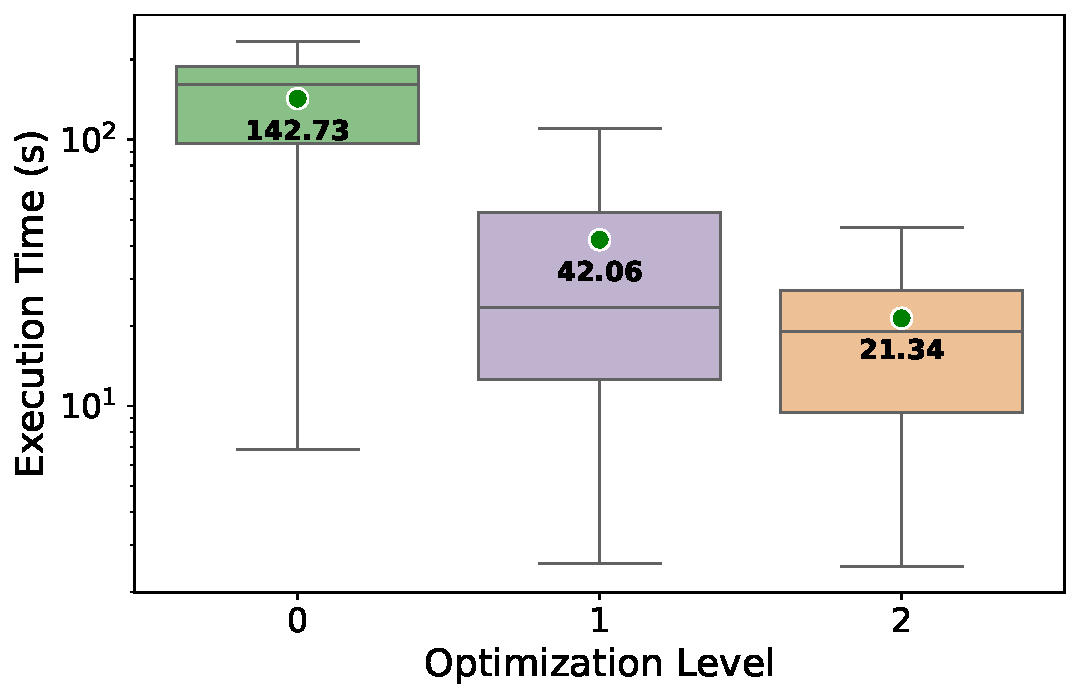
\includegraphics[width=\textwidth]{imgs/opt-bench.pdf}
		\caption{Across different optimization levels}
		\label{fig:result-opt-performance}
	\end{subfigure}
	\hspace{1em}
	\begin{subfigure}{0.48\textwidth}
		\centering
		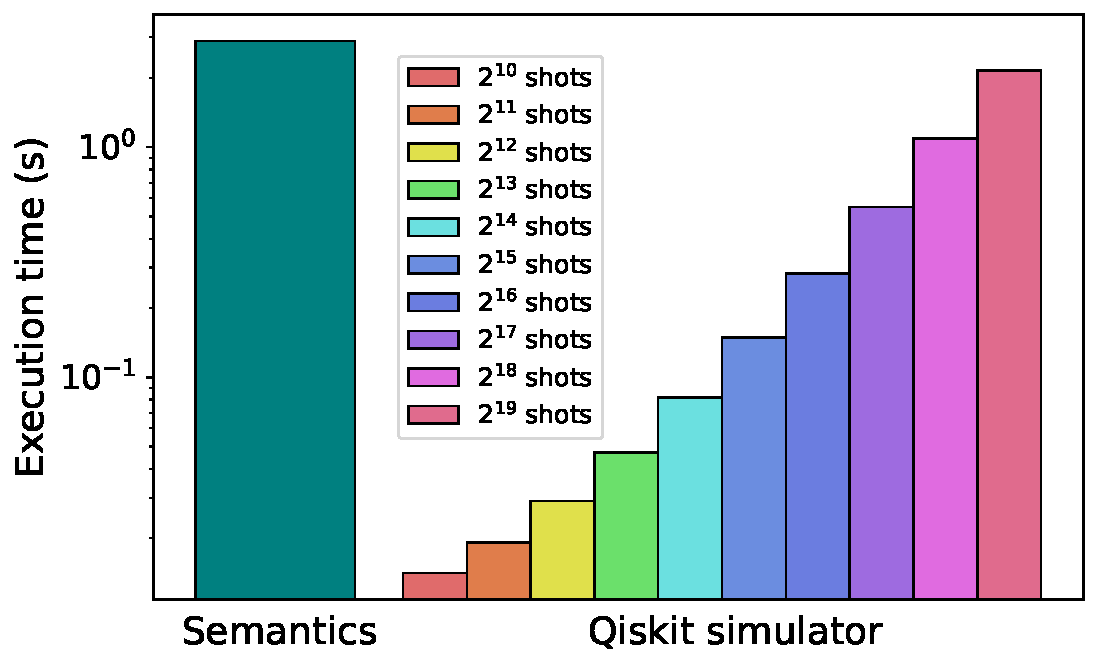
\includegraphics[width=\textwidth]{imgs/sim-bench.pdf}
		\caption{Semantics vs. Qiskit's simulator}
		\label{fig:result-performance}
		\vspace{0.9em}
	\end{subfigure}
	\caption{Execution times of OpenQASM circuits (log scale)}
\end{figure}

\section{RQ1: Effectiveness of Optimizations}
\label{ch:evaluation:rq1}

\noindent
We evaluate the effectiveness of the optimizations in reducing execution times
by comparing three settings: Level 0 (no optimizations), Level 1 (with world
merging), and Level 2 (both optimizations).
%
These optimizations particularly decrease the execution times of dynamic
circuits, which perform mid-circuit measurements, by reducing the creation of
new worlds during measurements.
%
Due to the scarcity of dynamic circuits in available OpenQASM benchmark suites,
we generated 100 random dynamic circuits and used them for evaluation.
%
Each circuit comprises five qubits and average 62.8 random operations, where
each operation is either a reset, a measurement, or a gate chosen from Qiskit's
built-in gate set, consisting of 52 different gates.
%
Additionally, each operation has a 50\% chance of being conditional.
%
By properly setting the probability of selecting each operation, each circuit
has 5.7 measurements and 4.9 resets on average.

Our experimental results indicate a significant reduction in execution times
due to these optimizations.
%
\cref{fig:result-opt-performance} shows a box plot of the execution times across
different settings, with green dots representing average times, annotated in
black text.
%
Two optimizations collectively achieve an average reduction of 85\%.
%
Specifically, world merging achieves an average reduction of 71\%, while
efficient reset leads to a 49\% reduction.
%
World merging is more effective because it can be applied to any statements,
which may create two worlds with the same classical state.
%
This technique would be especially effective in circuits with measurements
considerably more than classical bits, as it limits the number of worlds
regardless of the number of measurements.
%
In contrast, unlike the typical reset, efficient reset does not exponentially
increase the number of worlds with each reset.
%
This benefit exponentially grows with the number of reset statements, making
efficient reset particularly effective for circuits with frequent resets.

To better understand the performance characteristics of the semantics, we
further compare its execution times with those of a real-world simulator.
%
We utilized \C{aer\_simulator} from Qiskit, with parallel execution disabled.
%
For this experiment, we employed 141 circuits from three benchmark suites, in
addition to the 100 randomly generated dynamic circuits.
%
The first suite is OpenQASM 2.0 specification~\cite{openqasm2}, where we
selected six example circuits by excluding one with ten qubits.
%
The second suite is QASMBench~\cite{li2023qasmbench}, where we selected 35
circuits from 81 by excluding those with nine or more qubits and one with eight
qubits.
%
The third suite, Supermarq~\cite{tomesh2022supermarq}, offers eight benchmark
generators, from which we generated 100 circuits.
%
Details on the simulator names and circuit sizes are available in the companion
report~\cite{supp}.

To compare performance, we executed the semantics only once for each circuit,
while we executed the simulator multiple times for each circuit.
%
This approach stems from the fact that our semantics computes the exact
probability distribution, eliminating the need for repeated runs.
%
In contrast, the simulator yields a nondeterministic outcome in each execution,
requiring multiple runs to approximate the probability distribution.

\cref{fig:result-performance} presents the geometric mean of execution times for
the circuits using each method: our semantics with optimization Level 2 or
\C{aer\_simulator}.
%
We employ the geometric mean due to significant variances in execution times
across circuits, with the slowest being 100,000 times longer than the fastest.
%
The left bar in the figure indicates the execution time for the semantics,
while the right bars represent the simulator's execution times, varying by the
number of runs.
%
The results demonstrate that a single semantics run is roughly equivalent in
time to $2^{19}$ simulator runs.
%
However, this does not imply that the semantics' performance is exceedingly
poor, as its capabilities fundamentally differ from those of the simulators,
which cannot compute the exact probability distribution regardless of the
number of runs.

\section{RQ2: Effectiveness as a Tesing Oracle}
\label{ch:evaluation:rq2}

\noindent
To evaluate the effectiveness of our semantics as a testing oracle, we tested a
simulator, \C{aer\_simulator}, provided by Qiskit using the semantics.
%
Simulating an OpenQASM circuit in Qiskit involves three steps:
%
(1) transpilation, which converts OpenQASM code into a circuit in Qiskit's
internal representation,
%
(2) optional optimization passes that transform the circuit, and
%
(3) simulation, which executes the circuit using a simulator.
%
By saying ``we tested a simulator,'' we mean testing all three steps, with the
simulator employed in the third step.
%
We tested steps 2 and 3 separately for effectiveness, utilizing step 1 in both
cases, as steps 2 and 3 rely on step 1.

To test optimization passes with an OpenQASM circuit, we first transpile (step
1) and optimize (step 2) the circuit, with all optimization passes enabled.
%
We then convert the optimized circuit back to OpenQASM code and execute both
the original and the optimized OpenQASM circuits using the semantics.
%
Finally, we compare the resulting probability distributions from both
executions, and any discrepancy indicates a bug in the optimization passes.

To generate circuits that trigger as many optimizations as possible, we
examined the optimization passes and developed a circuit generator tailored to
this task.
%
Below are all the optimization passes in Qiskit, except for
\C{CrosstalkAdaptiveSchedule}, along with the operations we insert into
circuits to activate them.
%
The \C{CrosstalkAdaptiveSchedule} pass is excluded because it optimizes
circuits based on a user-provided hardware description.
%
\begin{itemize}[leftmargin=*]
	%
	\item \C{collect\_cliffords}/\C{collect\_linear\_functions}:
	      %
	      Each of them replaces a block of Clifford/linear gates with a single gate.
	      %
	      We insert a block of Clifford/linear gates.
	      %
	\item \C{commutative\_cancellation}:
	      %
	      It removes a pair of adjacent gates that are self-inverse.
	      %
	      We insert a sequence of self-inverse gates.
	      %
	\item \C{commutative\_inverse\_cancellation}:
	      %
	      It removes a pair of possibly non-adjacent inverse gates by exploiting
	      commutation relations.
	      %
	      We insert a sequence consisting of an arbitrary gate at the beginning, its
	      inverse at the end, and gates commuting with them in between.
	      %
	\item \C{consolidate\_blocks}:
	      %
	      It replaces a sequence of consecutive gates with a single gate.
	      %
	      We insert a sequence of gates.
	      %
	\item \C{cx\_cancellation}:
	      %
	      It removes a pair of adjacent CNOT gates.
	      %
	      We insert a sequence of CNOT gates.
	      %
	\item \C{echo\_rzx\_weyl\_decomposition}:
	      %
	      It rewrites a two-qubit gate using the Weyl decomposition.
	      %
	      We insert a block of two-qubit gates.
	      %
	\item \C{hoare\_opt}:
	      %
	      It applies Hoare logic to selective gates.
	      %
	      We insert a block of gates handled by Hoare logic.
	      %
	\item \C{inverse\_cancellation}:
	      %
	      It removes a pair of adjacent inverse gates.
	      %
	      We insert an arbitrary gate and its inverse. \item
	      \C{optimize\_1q\_commutation}:
	      %
	      It optimizes the circuit by exploiting a 1-qubit gate commuting with a 2-qubit
	      gate.
	      %
	      We insert a 2-qubit gate and a 1-qubit gate commuting with it.
	      %
	\item \C{optimize\_cliffords}:
	      %
	      It replaces a sequence of consecutive Clifford gates over the same qubit with a
	      single gate.
	      %
	      We insert a sequence of Clifford gates over a single qubit.
	      %
	\item \C{optimize\_swap\_before\_measure}:
	      %
	      It removes a SWAP gate followed by a measurement.
	      %
	      We insert a SWAP gate followed by a measurement.
	      %
	\item \C{remove\_diagonal\_gates\_before\_measure}:
	      %
	      It removes a diagonal gate followed by a measurement.
	      %
	      We insert a diagonal gate followed by a measurement.
	      %
	\item \C{remove\_reset\_in\_zero\_state}:
	      %
	      It removes a reset on a qubit in $\ket{0}$ state.
	      %
	      We insert a reset on a qubit in $\ket{0}$ state.
	      %
	\item \C{reset\_after\_measure\_simplification}:
	      %
	      It removes a reset preceded by a measurement.
	      %
	      We insert a reset preceded by a measurement.
	      %
\end{itemize}

To test simulation with an OpenQASM circuit, we transpile (step 1) and then
simulate (step 3) the circuit, with all optimization passes disabled.
%
As the simulator is sampling-based and produces nondeterministic results, we
must compare the outcomes from multiple simulator runs to the probability
distribution computed by the semantics.
%
For this comparison, we employ the chi-square goodness-of-fit
test~\cite{pearson1900criterion}.
%
This test evaluates whether observed outcomes are likely sampled from a given
probability distribution.
%
The p-value computed by the test indicates the likelihood of the observed
outcomes occurring if the null hypothesis (the observations are sampled from
the distribution) is true.
%
A low p-value suggests that the outcomes are improbable under the null
hypothesis, strongly indicating that the observations do not conform to the
expected probability distribution.
%
Consistent with standard statistical hypothesis testing practices, we interpret
a p-value below 0.01 (=1\%) as evidence of divergence between the semantics and
the simulator.

\begin{table}[t]
	\centering
	\caption{Real-world bugs found by our approach}
	\label{table:bugs}
	{\footnotesize
		\begin{tabular}{@{}lllllll@{}}
			\toprule
			ID    & Location      & Platform & Status    & Novelty   & Description                                   \\ \midrule
			Bug 1 & transpilation & Qiskit   & fixed     & new       & losing classical conditionals                 \\
			Bug 2 & optimization  & Qiskit   & fixed     & duplicate & wrong commutation analysis                    \\
			Bug 3 & optimization  & Qiskit   & confirmed & new       & incorrectly optimizing SWAP and measurement   \\
			Bug 4 & optimization  & Qiskit   & confirmed & new       & Hoare optimizer ignoring classical conditions \\
			Bug 5 & optimization  & Qiskit   & confirmed & new       & Hoare optimizer misusing gate cancellation    \\
			Bug 6 & optimization  & staq     & fixed     & new       & losing conditionals                           \\ \bottomrule
		\end{tabular}
	}
\end{table}

Our results demonstrate the effectiveness of the semantics as a testing oracle.
%
We generated 40,000 static circuits and 10,000 dynamic circuits using the
optimization-triggering circuit generator to test both optimization and
simulation.
%
When testing simulation, we ran the simulator 1,024 times for each circuit.
%
From testing, we discovered five bugs in Qiskit, detailed as Bugs 1 to 5 in
\cref{table:bugs}.
%
To the best of our knowledge, this is the first systematic testing to identify
bugs pertained to physical inconsistencies within real-world quantum
programming platforms.

These bugs were identified through optimization testing, with Bug 1 also
detected during simulation testing as it is due to incorrect transpilation.
%
Initially, out of 50,000 circuits, 10,000 (all the dynamic circuits) failed in
optimization testing, and 9,037 yielded p-values below 0.01 in simulation
testing.
%
A manual examination of a few circuits revealed Bug 1.
%
As Bug 1 led to numerous failures, hindering the discovery of other bugs, we
repeated the optimization and simulation testing after fixing Bug 1.
%
This resulted in 2,716 failures in optimization testing and a few circuits with
p-values below 0.01 in simulation testing.
%
Further manual investigation of the failed circuits in optimization testing
identified Bugs 2 to 5:
%
30 failures caused by Bug 2, 99 by Bug 3, 2,586 probably caused by Bug 4, and 1
by Bug 5.
%
While we cannot manually analyze all 2,586 failures, they have conditionals and
persist even when only the \C{hoare\_opt} pass is enabled, leading us to
suspect that all are attributable to Bug 4.
%
Conversely, no additional bugs were identified from circuits with low p-values,
which is consistent with the expectation that approximately 0.01\% of the
circuits should exhibit p-values below 0.01, by definition of a p-value.

Of the identified bugs, four, excluding Bug 2, were previously unknown.
%
Bug 2, although not fixed in the latest release of Qiskit used for our
experiments, had been identified and fixed in the development version.
%
We reported the four new bugs, which were all confirmed by the Qiskit
developers, and Bug 1 was fixed subsequent to our report.

We also conducted experiments with staq, an open-source library for quantum
circuits~\cite{staq}.
%
Since staq provides optimizers but not simulators, we limited our tests to
optimization using the same 50,000 generated circuits.
%
In staq v3.3, we found one previously unknown bug, referred to as Bug 6 in
\cref{table:bugs}, which was subsequently confirmed and fixed by the staq
developers.
%
The circuits used for the experiment are specifically designed for testing the
optimization passes in Qiskit.
%
Therefore, designing a circuit generator tailored for staq's optimization
passes would reveal additional bugs.

\begin{figure}[t]
	\centering
	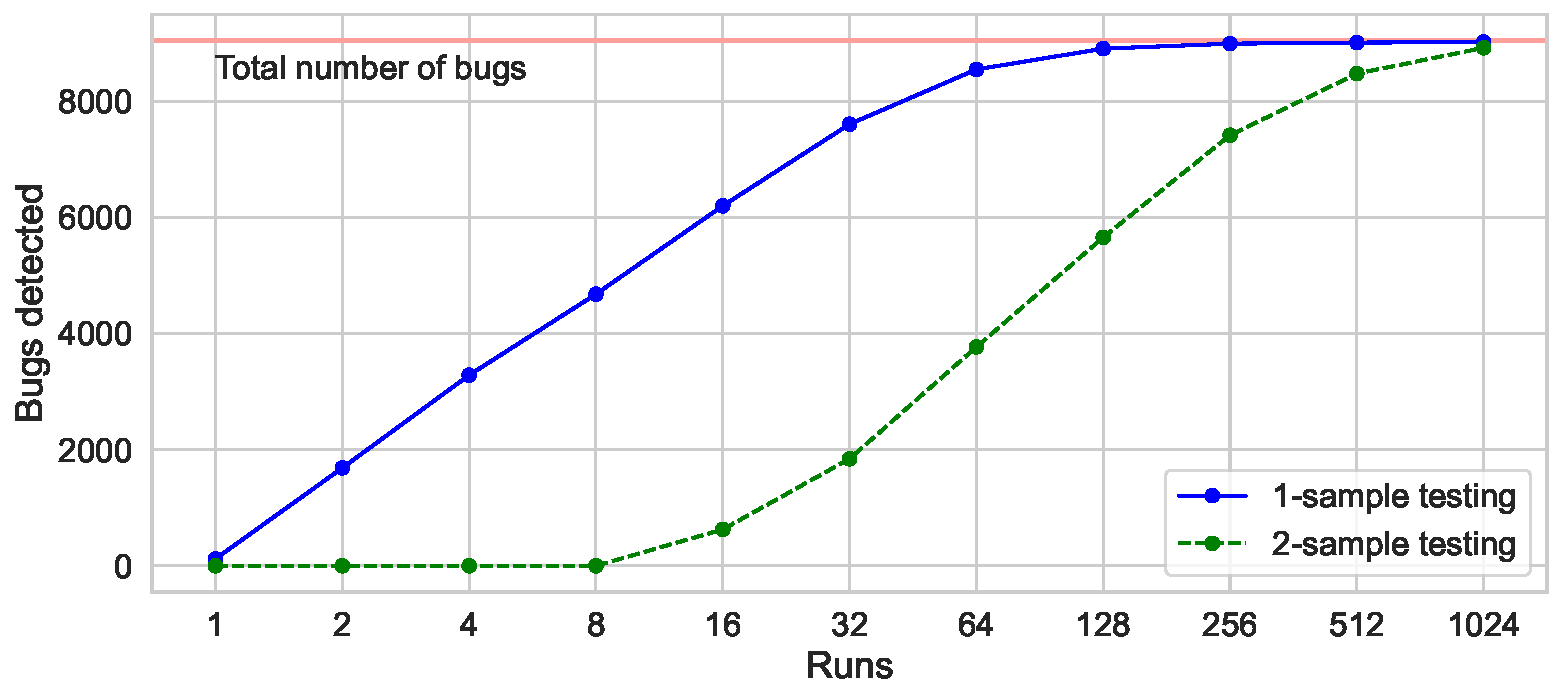
\includegraphics[width=0.64\textwidth]{imgs/1-2-sample-test.pdf}
	\caption{Number of detected bugs per number of simulator runs (x-axis is log scale)}
	\label{fig:onesample}
\end{figure}

We now compare testing simulation using the semantics to existing approaches to
test quantum circuit simulators, \textsc{QDiff}~\cite{wang2022qdiff} and
MorphQ~\cite{paltenghi2023morphq}.
%
\textsc{QDiff} employs a differential testing technique, executing the same
quantum circuit on multiple simulators and checking for output discrepancies.
%
MorphQ, in contrast, utilizes a metamorphic testing technique that generates
multiple semantically equivalent quantum circuits, executing them on a
simulator to compare their outputs.

At first glance, our method may appear similar to the existing ones, as both
methods compare independently-obtained results that should be identical if no
bugs exist.
%
However, our approach directly compares simulator outcomes with the probability
distribution computed by the semantics, known as the \emph{one-sample test} in
statistics.
%
In contrast, \textsc{QDiff} and MorphQ compare two sets of simulator outcomes
to determine if they are sampled from the same probability distribution,
referred to as the \emph{two-sample test}.
%
This distinction arises from the absence of a testing oracle computing the
probability distribution in their approaches.

Our case study demonstrates that our method can detect bugs with significantly
fewer simulator runs than existing approaches, due to the difference in
statistical confidence between one-sample and two-sample tests.
%
We utilized the 9,037 circuits affected by Bug 1 for this study.
%
For varying values of $N$, ranging from 1 to 1,024, we executed each circuit on
the simulator $N$ times.
%
The outcomes were compared with the probability distribution computed by the
semantics using the one-sample test.
%
Additionally, we ran the circuit on the corrected version of the simulator $N$
times, comparing the two sets of outcomes using the two-sample test.
%
In both tests, a p-value below 0.01 indicates successful bug detection.
%
\cref{fig:onesample} presents the results, illustrating that the one-sample test
is more effective than the two-sample test.
%
The x-axis represents $N$, while the y-axis shows the number of circuits in
which Bug 1 is detected.
%
As a larger sample size increases statistical confidence and lowers the
p-value, larger $N$ leads to the discovery of bugs across more circuits.
%
However, regardless of $N$, the one-sample test finds bugs in more circuits
than the two-sample test.

When testing optimization, our approach is even more advantageous than existing
methods.
%
Our method can directly compare distributions without any sampling, while
existing approaches must still rely on the less efficient two-sample test.


% !TEX root = main.tex

\chapter{Related Work}
\label{ch:related}

\paragraph{Formal Semantics for Programming Languages}

Researchers have defined formal semantics for various real-world programming
languages.
%
\Cref{ch:intro} already provides the list of studies of formal
semantics for each language.
%
Therefore, this section emphasizes their methodologies and compares them with
the approach proposed in this work.

While numerous studies have directly defined the formal semantics of a complete
real-world language, this approach necessitates significant manual effort.
%
To circumvent this issue, some studies have chosen to define formal semantics
by defining a small core language and then desugaring the surface language to
the core
language~\cite{guha2010essence,politz2012tested,memarian2016depths,politz2013python}.
%
This approach aligns with our work, where we introduce OpenQASMCore and perform
desugaring from OpenQASM to OpenQASMCore.

Another way to reduce the burden of defining formal semantics is to utilize
semantic frameworks, such as K~\cite{rosu2010overview}, PLT
Redex~\cite{felleisen2009semantics}, and Lem~\cite{mulligan2014lem}.
%
These semantic frameworks are also beneficial because they allow the semantics
to be executable without any additional work.
%
K is a rewrite-based semantic framework, in which the semantics of many
languages have been
formalized~\cite{park2015kjs,ellison2012executable,bogdanas2015kjava,filaretti2014executable,jiao2020semantic}.
%
PLT Redex is a domain-specific language for specifying operational semantics
and has been used to describe the semantics of various
languages~\cite{guha2010essence,politz2013python}.

Researchers have defined formal semantics using proof assistants as well.
%
Coq~\cite{barras1997coq} has been widely employed to mechanize formal
semantics~\cite{bodin2014trusted,blazy2009mechanized,jung2017rustbelt,watt2021two}.
%
Isabelle/HOL~\cite{nipkow2002isabelle} is another popular proof assistant used
for defining formal semantics~\cite{klein2006machine,watt2018mechanising}.
%
Semantics defined with proof assistants are often executable, such as shown by
\citet{bodin2014trusted}, who extract OCaml code from Coq.
%
In this work, we also mechanize the semantics in Coq and extract OCaml code.

One notable approach to obtaining formal semantics with low manual effort is to
automatically extract mechanized semantics from a structured natural language
specification, as proposed and adopted in JavaScript by \citet{park2021jiset}.
%
However, this approach is not applicable to OpenQASM due to its lack of
sufficient structure in the specification.

When formal semantics is executable, it is a standard approach to validate its
conformance using existing test suites.
%
Most traditional programming languages provide official conformance test
suites, such as Test262~\cite{test262} for JavaScript and the Java
Compatibility Kit~\cite{jck} for Java.
%
However, quantum computing is still in its early stages, and OpenQASM 2.0 does
not have an official test suite.
%
Consequently, we assess the conformance of the semantics using example circuits
from the OpenQASM 2.0 specification~\cite{openqasm2} and benchmark circuits
from QASMBench~\cite{li2023qasmbench}.
%
Several studies have demonstrated the practical utility of executable semantics
in identifying bugs in language
implementations~\cite{watt2023wasmref,schumi2021spectest,park2021jest} and
automatically generating test suites of high coverage~\cite{park2023feature}.

\paragraph{Quantum Programming Languages}

Researchers have proposed high-level quantum programming languages, which are
complementary to quantum circuit description languages, such as OpenQASM, the
main focus of this work.
%
While high-level languages allow programmers to express complex quantum
algorithms using abstractions, circuit description languages are tightly
coupled with real quantum hardware and often serve as the compilation targets
for high-level languages.

In the early days of quantum computing, quantum programming languages were
defined by incorporating quantum computations into classical languages.
%
For instance, QCL~\cite{omer2003structured} and qGCL~\cite{sanders2000quantum}
introduce imperative features alongside quantum computations, while quantum
lambda calculus~\cite{maymin1997extending},
QML~\cite{altenkirch2005functional}, and Quipper~\cite{green2013quipper} enable
quantum computations within functional languages.

Recently, researchers have proposed quantum programming languages to address
specific difficulties in quantum programming.
%
Here, we discuss a few notable examples.
%
Silq~\cite{bichsel2020silq} enables programmers to safely and concisely perform
\emph{uncomputation}, which means ignoring temporary qubits during computation
without any side effects.
%
Twist~\cite{yuan2022twist} aids in reasoning about \emph{purity}, i.e., the
absence of entanglement, through its novel type system.
%
Tower~\cite{yuan2022tower} allows the use of random-access memory for
implementing pointer-based data structures.
%
Qunity~\cite{voichick2023qunity} generalizes language constructs in classical
programming, thereby establishing a unified approach to quantum and classical
computing.
%
\citet{Feng2021Hoare} propose a Hoare logic for quantum programs by defining
classical-quantum states, which are capable of describing states of dynamic
circuits.
%
\textsc{voqc}~\cite{Hietala2021voqc} is the first verified optimizer for quantum
circuits, utilizing a language called \textsc{sqir}, compatible with OpenQASM.
%
Embedded in Coq, \textsc{sqir} facilitates the verification of \textsc{voqc}'s
correctness.

A notable exception is the work of \citet{paykin2017qwire}, which introduces
\textsc{Qwire}, a quantum circuit description language that can be manipulated
using a classical language.
%
Like our semantics, \textsc{Qwire}'s semantics is defined in terms of density
matrices.
%
Its type system guarantees the preservation of the trace of the density matrix,
ensuring that any well-typed circuit maintains a trace of 1 during execution.
%
This aligns with the last condition specified by \cref{pos:density}.
%
However, \textsc{Qwire} does not enforce the other properties required by the
density matrix postulate, whereas in this work, we prove the physical
consistency of the proposed semantics.

\paragraph{Testing Quantum Programming Platforms}

As mentioned in \Cref{ch:evaluation:rq2}, \textsc{QDiff}~\cite{wang2022qdiff}
and MorphQ~\cite{paltenghi2023morphq} are differential testing and metamorphic
testing techniques for quantum programming platforms, respectively.
%
Although these techniques are effective in identifying bugs in quantum
programming platforms, all the identified bugs are due to software crashes, but
not due to outcomes not following the correct probability distributions.
%
These approaches do not utilize a testing oracle to compute the correct
probability distributions, thereby limiting their bug detection capabilities.

% !TEX root = main.tex
\chapter{Conclusion}
\label{ch:conclusion}

\noindent
In this work, we propose the first executable formal semantics for OpenQASM
2.0, a representative quantum circuit description language.
%
To address the nondeterministic nature of quantum circuits, our semantics
computes the probability distribution of possible outcomes.
%
We adopt MWI from the physics literature to compute the probability
distribution even for dynamic quantum circuits and optimize the semantics using
mixed states.
%
Additionally, we prove the physical consistency of the semantics, which implies
adherence to the postulates of quantum mechanics.
%
To simplify the proof, we define OpenQASMCore as a core language of OpenQASM
and desugar OpenQASM to OpenQASMCore.
%
Our evaluation demonstrates the effectiveness of the optimizations in improving
performance and the utility of the semantics as a testing oracle, finding five
previously unknown bugs in two real-world quantum computing platforms.


\chapter[Method]{Method}
\label{ch:ourmethod}
\section{Quantum Communication}
To enhance the performance gain of original cognitive radio networks (CRNs),
leveraging cooperative diversity has attracted a lot of attention
\cite{SOCA1}...

\section{Examples}

\section{Applications of Quantum Communication}
\label{ch:application}
\noindent
Despite its potential to improve the throughput, spatial domain diversity was not fully considered in the studies of original CCRNs. Utilizing the spatial domain for the communications, the concept of MIMO has been adopted in many cases to increase the wireless capacity \cite{EF1,FD2}...

Let us consider an MIMO-CCRN with one PL and one SL. Each PU has one legacy
antenna and each SU has two STAR antennas. The duration of one communication
time frame is divided into two phases \cite{RVP2,ML2} ...
%%
%% 표 삽입 예시
%% Example. how to insert table
%%
\begin{table}[t]
	\caption[Enter the caption title here]{Energy stability $E$ (eV) per molecule of all meta-stable
		isomer states of C$_{60}$ opening process for forming the (5,5) cap.
		In the SW-I and SW-II, both ferromagnetic (Ferro) and paramagnetic (Para)
		spin configurations are obtained, whereas only non-magnetic configuration
		is obtained in the BF, SW-III, and CAP(5,5).
		$M$ is total magnetization $n_{\rm up}$-$n_{\rm down}$ in unit of $\mu_B$, where
		$n_{\rm up(down)}$ is the number of up (down) spins.
	}
	\label{mag-tab1}
	\begin{center}
		\begin{tabular} {ccccccccccc}
			\hline\hline
			 &               & BF & \multicolumn{2}{c}{SW-I} &       & \multicolumn{2}{c}{SW-II} & SW-III & CAP    &               \\
			\cline{4-5} \cline{7-8}
			 &               &    & Para                     & Ferro &                           & Para   & Ferro  &      &      & \\
			\hline
			 & $E$ (eV)      & 0  & 7.796                    & 7.832 &                           & 10.418 & 10.408 & 11.5 & 13.2 & \\
			 & $M$ ($\mu_B$) & 0  & 0                        & 1.94  &                           & 0      & 2.06   & 0    & 0    & \\
			\hline\hline
		\end{tabular}
	\end{center}
\end{table}

%%
%% 그림 삽입 예시
%% Example. how to insert graph
%%
%% Note. 가급적 \includegraphics 명령을 사용하십시오.
%% Recommen : Use \includegraphics to insert graph.
%%
\begin{figure}[t]
	\centerline{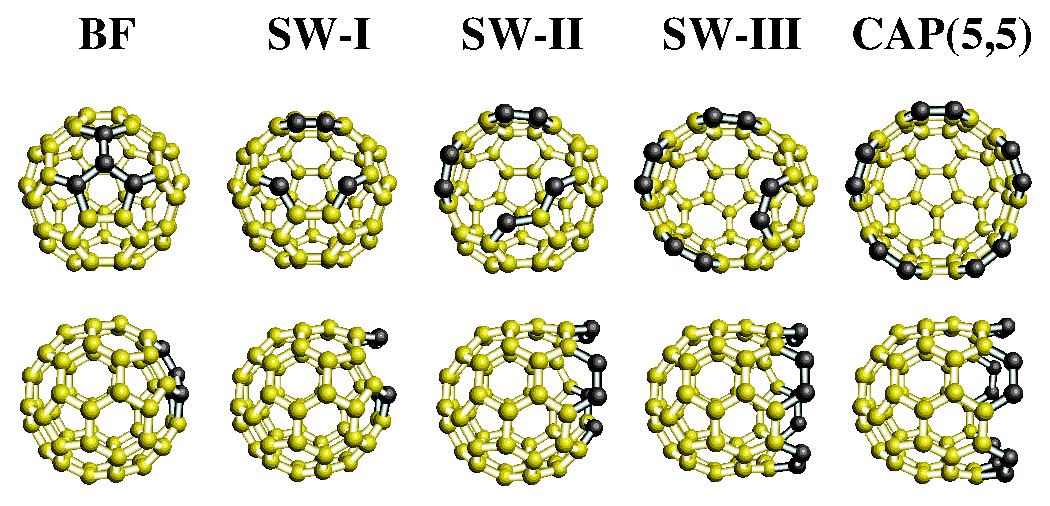
\includegraphics[width=12.5cm]{sample-fig1}}
	\caption[Enter the caption title here]{ Ball-and-stick models of meta-stable isomers in
		cage opening process from a C$_{60}$ buckminsterfullerene
		to a (5,5) capsule. We name them BF and CAP(5,5).
		Depending on the number of the Stone-Wales (SW) transformation,
		we call the intermediate isomers with SW-I, SW-II, and SW-III.
		Highlighted atoms are undercoordinated except BF.
	} \label{mag-fig1}
\end{figure}

\section{Discussion and Future Work}
\noindent
The achievable rates can be calculated by finding the statistics of the five signals transmitted that maximize the mutual information between $s_{t,XY}$ and $y_{t,XY}$ for $(X,Y)=(T,C), (C,N)$, and $(N,C)$ when $t=1$, and $(X,Y)=(C,R), (C,N)$, and $(N,C)$ when $t=2$ \cite{SOCA2,EF2}...

\chapter{Conclusion}
\noindent
We have proposed a novel FD MIMO-CCRN framework providing a reasonable performance improvement compared with the conventional MIMO-CCRN framework...
%%
%% 참고문헌 시작
%% bibliography
%% It can be changed but should include sufficient information.
% \bibliographystyle{abbrvnat}
\bibliographystyle{plainnat}
\bibliography{references}

%%
%% 감사의 글 시작
%% Acknowledgement
%%
% @command acknowledgement 감사의글
% @options [1 | 2 | 3 |4 ]
% - 1 : 본문과 감사의 글이 둘 다 한글일 때  | 2 : 본문은 한글인데 감사의 글이 영어일 때 | 3 :  본문과 감사의 글이 둘 다 영어일 때  | 4 : 본문은 영어인데 감사의 글이 % 한글일 때
%% It is optional.

\acknowledgment[4]
언제나 저를 바른 길로 이끌어 주시는 송익호 교수님께 큰 고마움을 느낍니다.
끝으로 오늘의 제가 있을 수 있도록 사랑으로 키워 주신 가족들에게 감사드립니다.
저의 이 작은 결실이 그분들께 조금이나마 보답이 되기를 바랍니다.

%%
%% 약력 시작
%% Curriculum Vitae
%%
% @command curriculumvitae 이력서
% @options [1 | 2 | 3 |4 ]
% - 1 : 본문과 약력이 둘 다 한글일 때  | 2 : 본문은 한글인데 약력이 영어일 때 | 3 :  본문과 약력이 둘 다 영어일 때  | 4 : 본문은 영어인데 약력이 한글일 때
%% It is optional and you can change form of this in the class file if you want.
\curriculumvitae[4]

% @environment personaldata 개인정보
% @command     name         이름
%              dateofbirth  생년월일
%              birthplace   출생지
%              domicile     본적지
%              address      주소지
%              email        E-mail 주소
% - 위 6개의 기본 필드 중에 이력서에 적고 싶은 정보를 입력
% input data only you want
\begin{personaldata}
	\name       {이 강 욱}
	\dateofbirth{1999}{08}{01}
	\birthplace {...}
	\address    {...}
\end{personaldata}

% @environment education 학력
% @options [default: (none)] - 수학기간을 입력
\begin{education}
	\item[2015. 3.\ --\ 2017. 2.] 고등학교 (2년 수료)
	\item[2017. 3.\ --\ 2022. 8.] 한국과학기술원 물리학과 (학사)
	\item[2022. 9.\ --\ 2024. 2.] 한국과학기술원 전산학부 (석사)
\end{education}

% @environment career 경력
% @options [default: (none)] - 해당기간을 입력
\begin{career}
	\item[2021. 3.\ --\ 2021. 8.] 쓰레기통 청소
\end{career}

% @environment activity 학회활동
% @options [default: (none)] - 활동내용을 입력
%%    \begin{activity}
%%        \item J. Choi, \textbf{Yong-Hyun Kim}, K.J. Chang, and D. Tomanek,
%%             \textit{Occurrence of itinerant ferromagnetism in C/BN superlattice
%%             nanotubes}, 5th Asian Workshop on First-Principles Electronic
%%             Structure Calculations, Seoul (Korea), October., 2002.
%%    \end{activity}

% @environment publication 연구업적
% @options [default: (none)] - 출판내용을 입력
\begin{publication}
	%\item \textbf{Yong-Hyun Kim}, J. Choi, K.J. Chang, and D. Tomanek,
	%     \textit{Magnetic instability in partly opened C$_{60}$ isomers},
	%     in preparation.
	\item H.-K. Min, Y. Hou, {\bf S. Park}, and I. Song, ``A computationally efficient
	scheme for feature extraction with kernel discriminant analysis," \textit{Patt.
		Recogn.}, vol.~50, no.~2, pp.~45-55, Feb. 2016 (to be published).
\end{publication}

\label{paperlastpagelabel}     % <-- 추가 부분: 마지막 페이지 위치 지정
%% 본문 끝
\end{document}
